% Supplementary Materials — 中文翻译（不含 \section 标签）
% 对应 main.tex 第 1990--2220 行 \section*{Supplementary Materials} 之后正文
\label{sec:supplementary}

本节对正文中引用的 60 张逐种子可靠性图进行编目。每张图展示了 60 个种子实验
（6 个迁移对 $\times$ 2 种架构 $\times$ 5 个种子）中某一个的校准曲线、
可靠性图以及 $\Delta$ECE 柱状图。各图命名为
\texttt{fig\_reliability\_supp\_\{pair\}\_\{arch\}\_seed\{s\}.pdf}，
并作为外部文件随投稿一并提交。

\subsection*{S1.\ 逐种子可靠性图}
\label{sec:supp-reliability}

这 60 张图按迁移对和架构组织。每张图对应主结果表中的一行，提供了正文中所报告
$\Delta$ECE 值背后的可视化校准证据。对每个方向，分别给出 ResNet1D 和
InceptionTime 在种子 42--46 上的可靠性图。

\subsubsection*{S1.1.\ Chapman$\rightarrow$CPSC}

\begin{figure}[h]
\centering
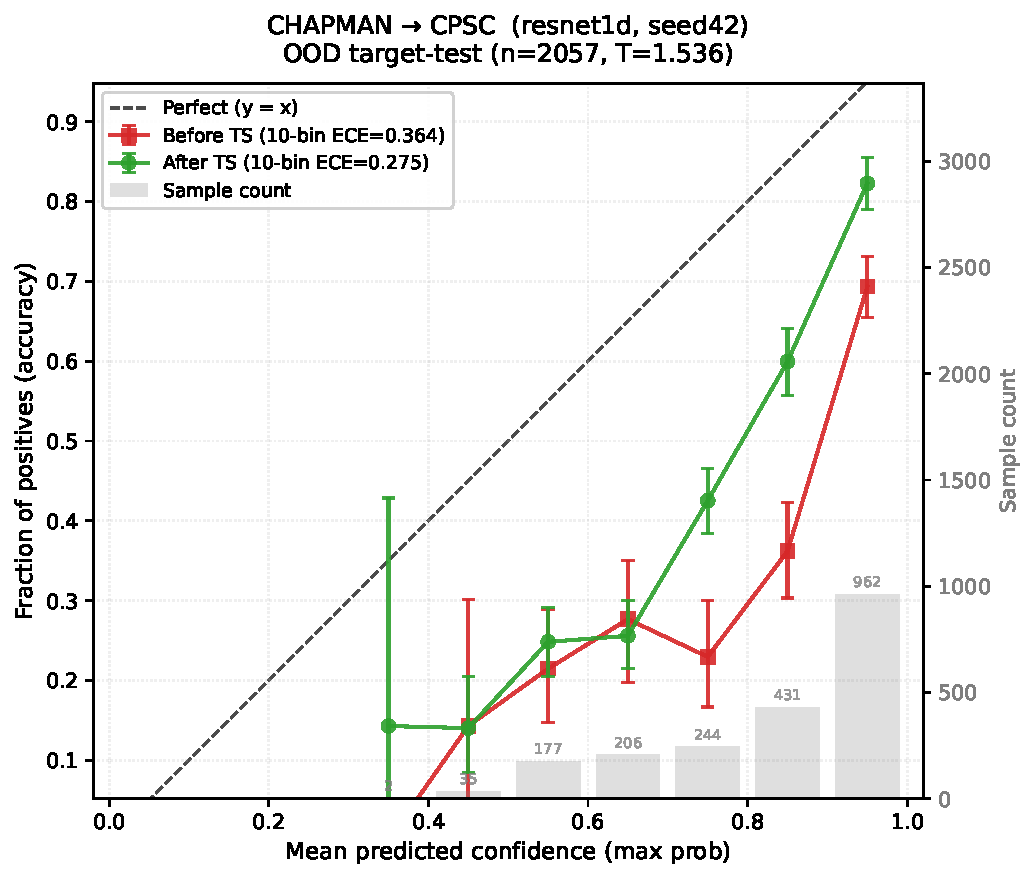
\includegraphics[width=0.32\textwidth]{figures/fig_reliability_supp_chapman_cpsc_resnet1d_seed42.pdf}
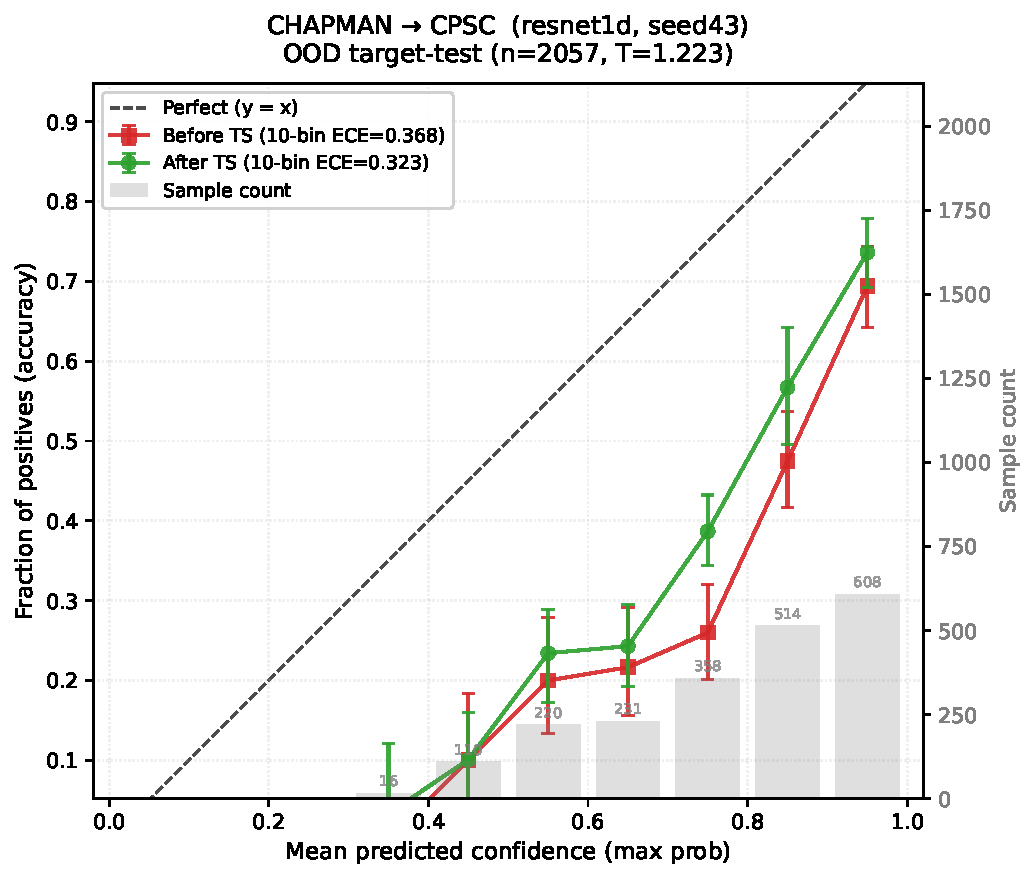
\includegraphics[width=0.32\textwidth]{figures/fig_reliability_supp_chapman_cpsc_resnet1d_seed43.pdf}
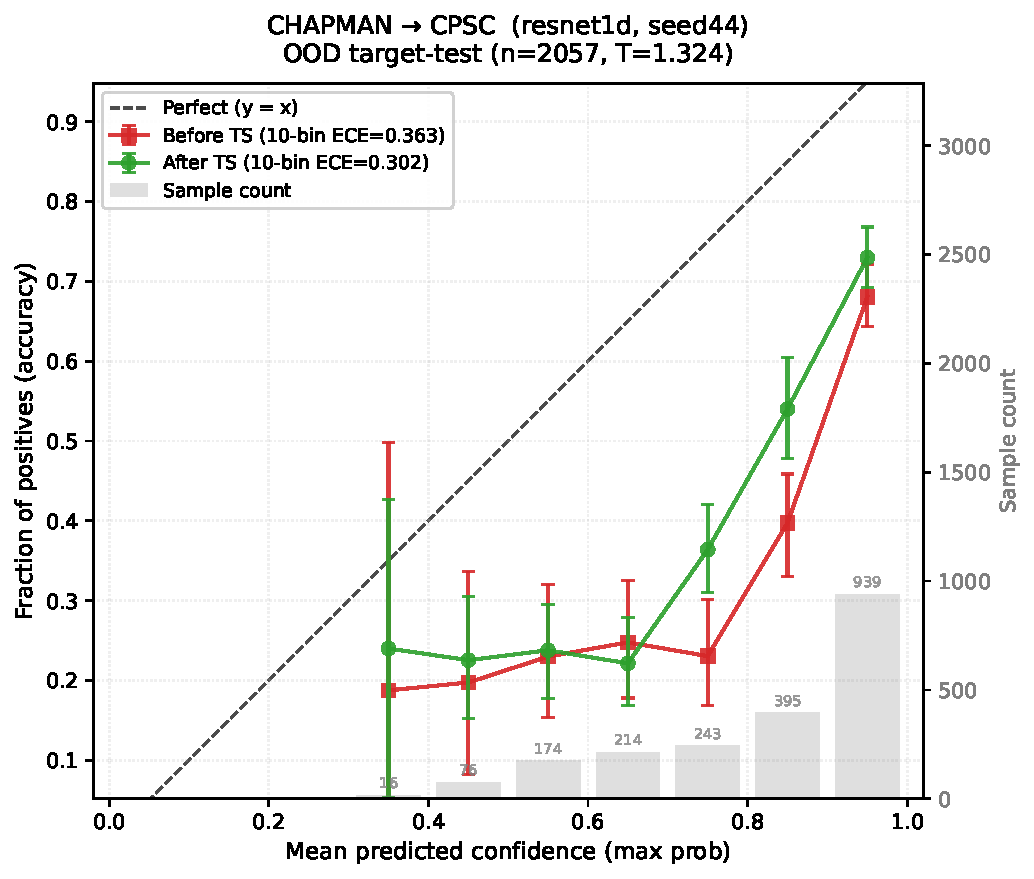
\includegraphics[width=0.32\textwidth]{figures/fig_reliability_supp_chapman_cpsc_resnet1d_seed44.pdf}
\caption{Chapman$\to$CPSC 可靠性图：ResNet1D 种子 42--44。}
\end{figure}

\begin{figure}[h]
\centering
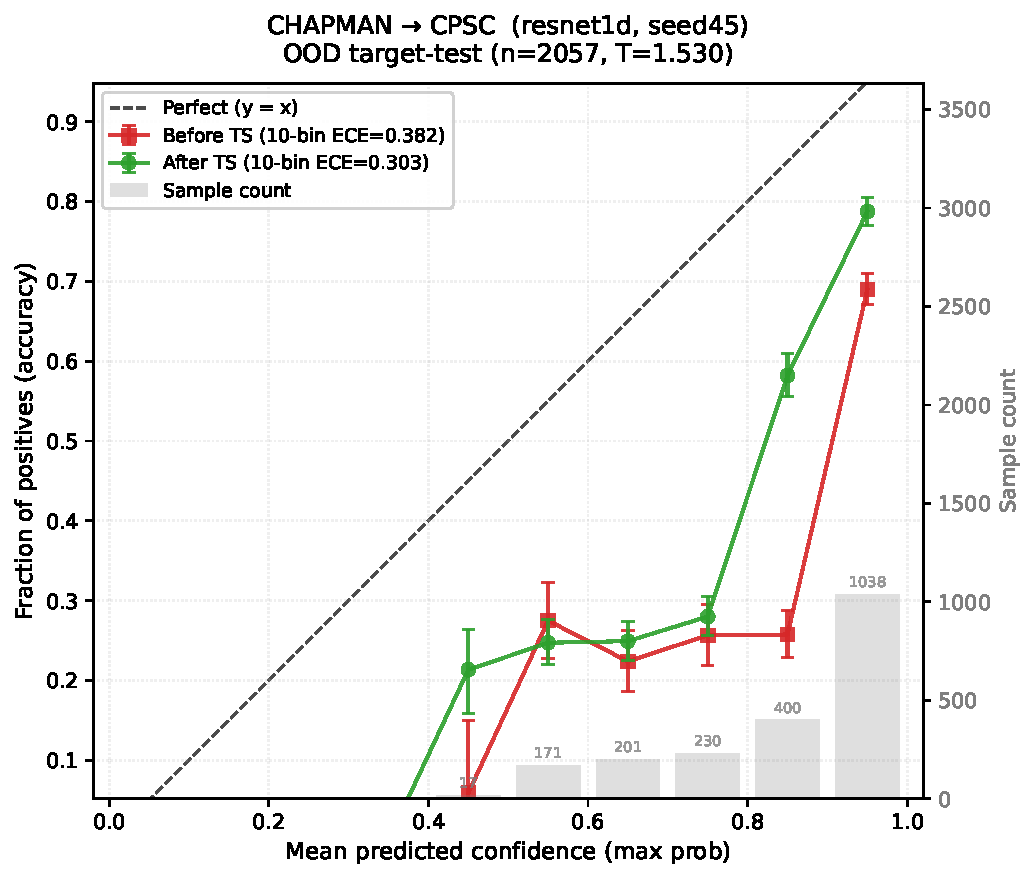
\includegraphics[width=0.45\textwidth]{figures/fig_reliability_supp_chapman_cpsc_resnet1d_seed45.pdf}
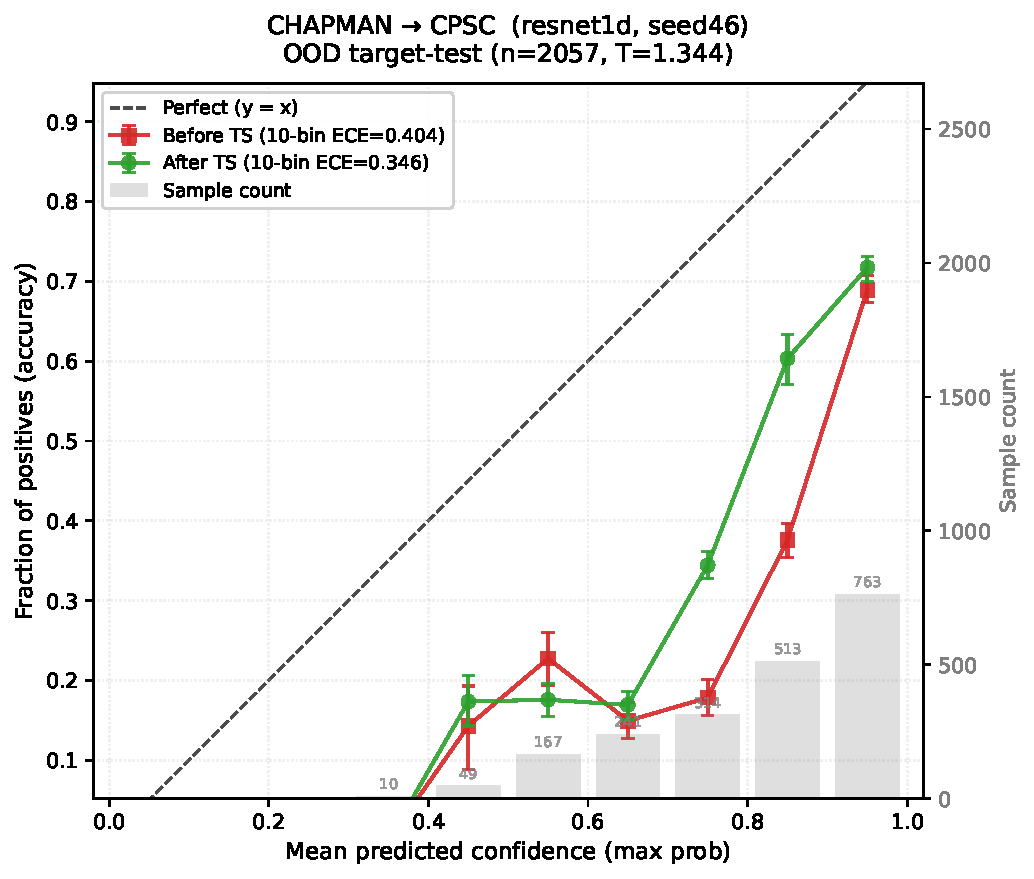
\includegraphics[width=0.45\textwidth]{figures/fig_reliability_supp_chapman_cpsc_resnet1d_seed46.pdf}
\caption{Chapman$\to$CPSC 可靠性图：ResNet1D 种子 45--46。}
\end{figure}

\begin{figure}[h]
\centering
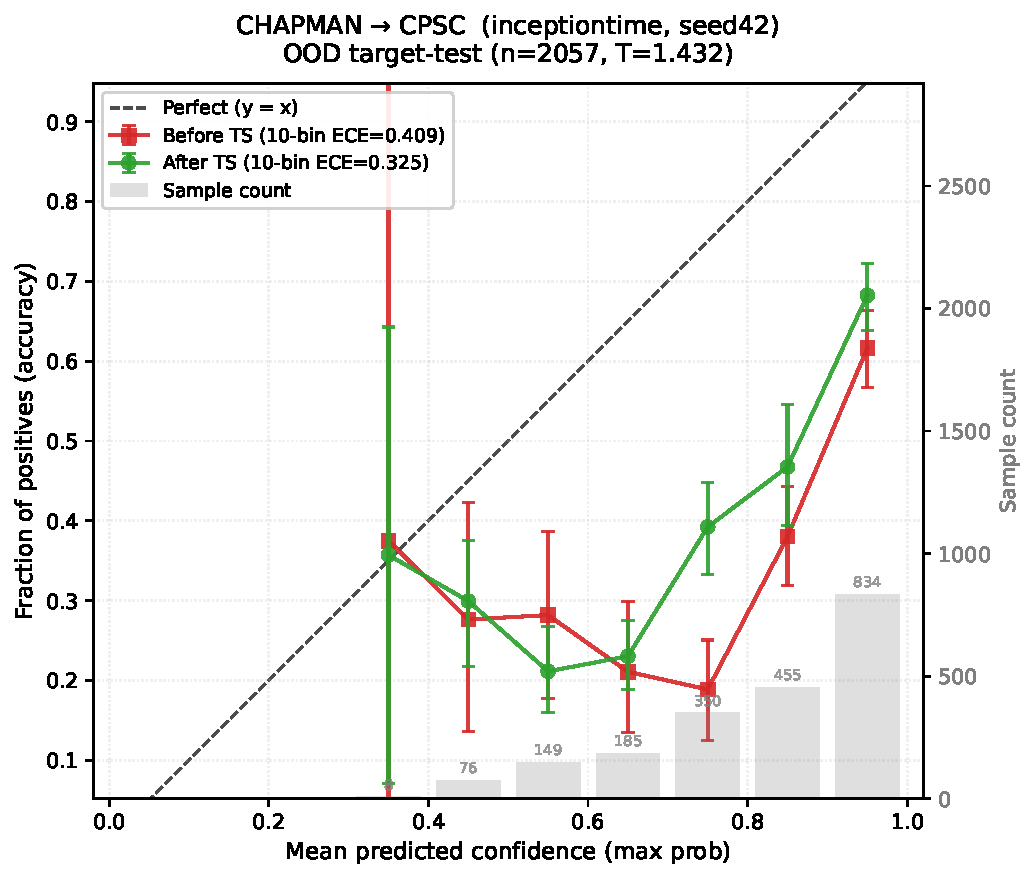
\includegraphics[width=0.32\textwidth]{figures/fig_reliability_supp_chapman_cpsc_inceptiontime_seed42.pdf}
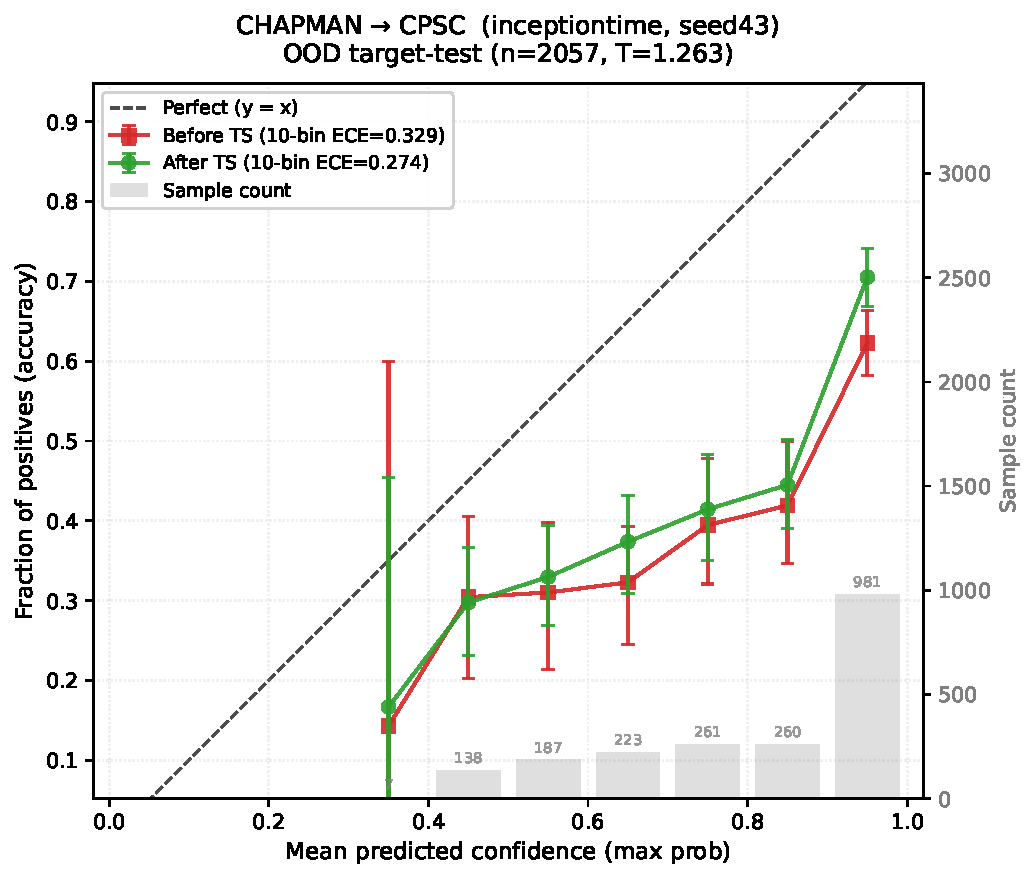
\includegraphics[width=0.32\textwidth]{figures/fig_reliability_supp_chapman_cpsc_inceptiontime_seed43.pdf}
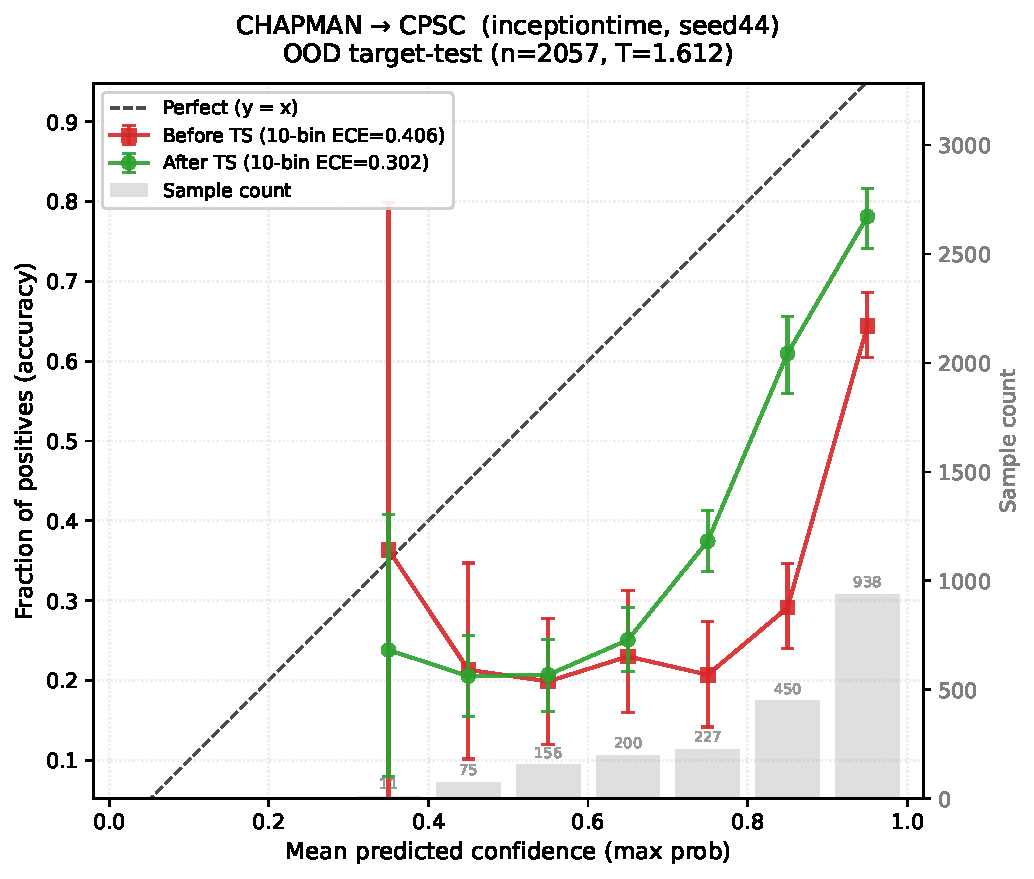
\includegraphics[width=0.32\textwidth]{figures/fig_reliability_supp_chapman_cpsc_inceptiontime_seed44.pdf}
\caption{Chapman$\to$CPSC 可靠性图：InceptionTime 种子 42--44。}
\end{figure}

\begin{figure}[h]
\centering
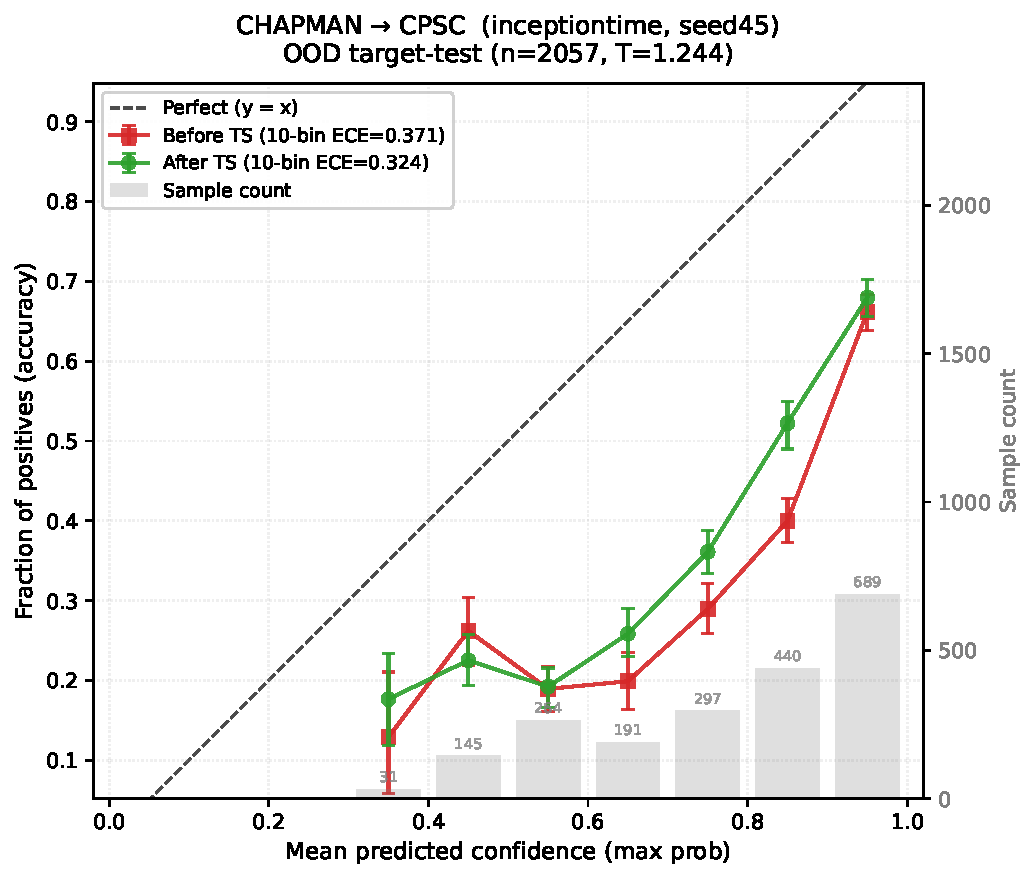
\includegraphics[width=0.45\textwidth]{figures/fig_reliability_supp_chapman_cpsc_inceptiontime_seed45.pdf}
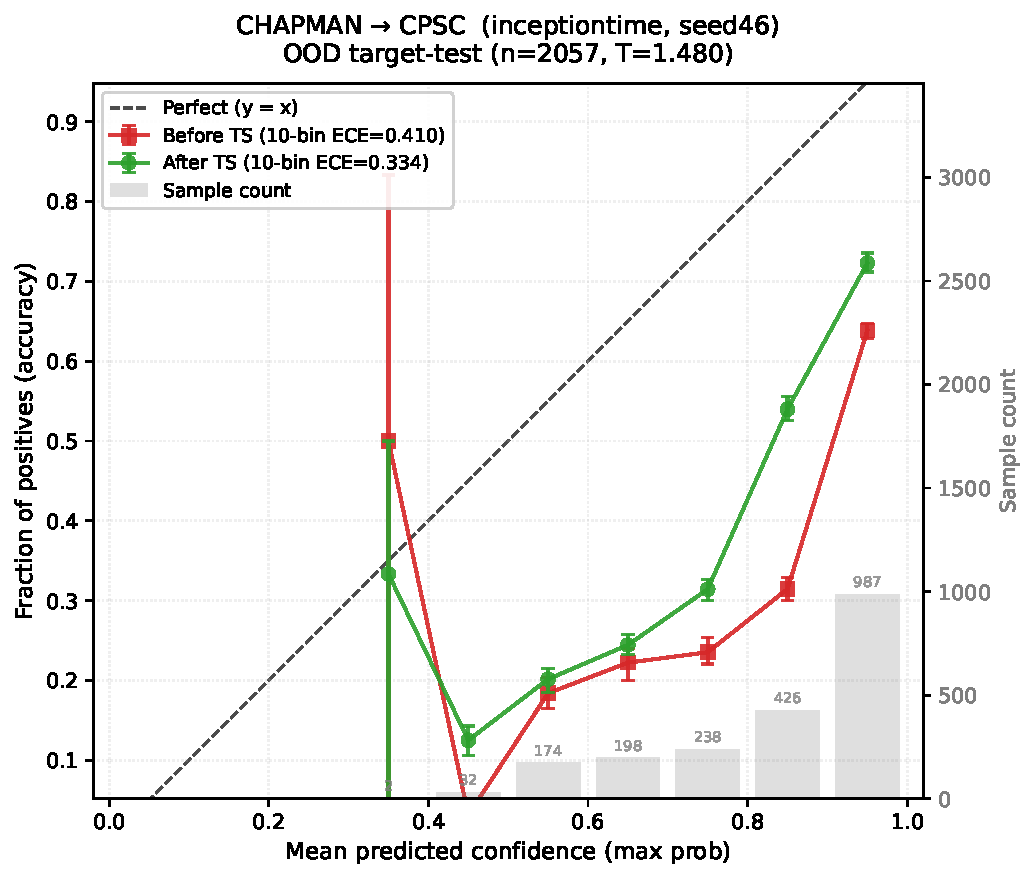
\includegraphics[width=0.45\textwidth]{figures/fig_reliability_supp_chapman_cpsc_inceptiontime_seed46.pdf}
\caption{Chapman$\to$CPSC 可靠性图：InceptionTime 种子 45--46。}
\end{figure}

\subsubsection*{S1.2.\ Chapman$\rightarrow$PTB-XL}

\begin{figure}[h]
\centering
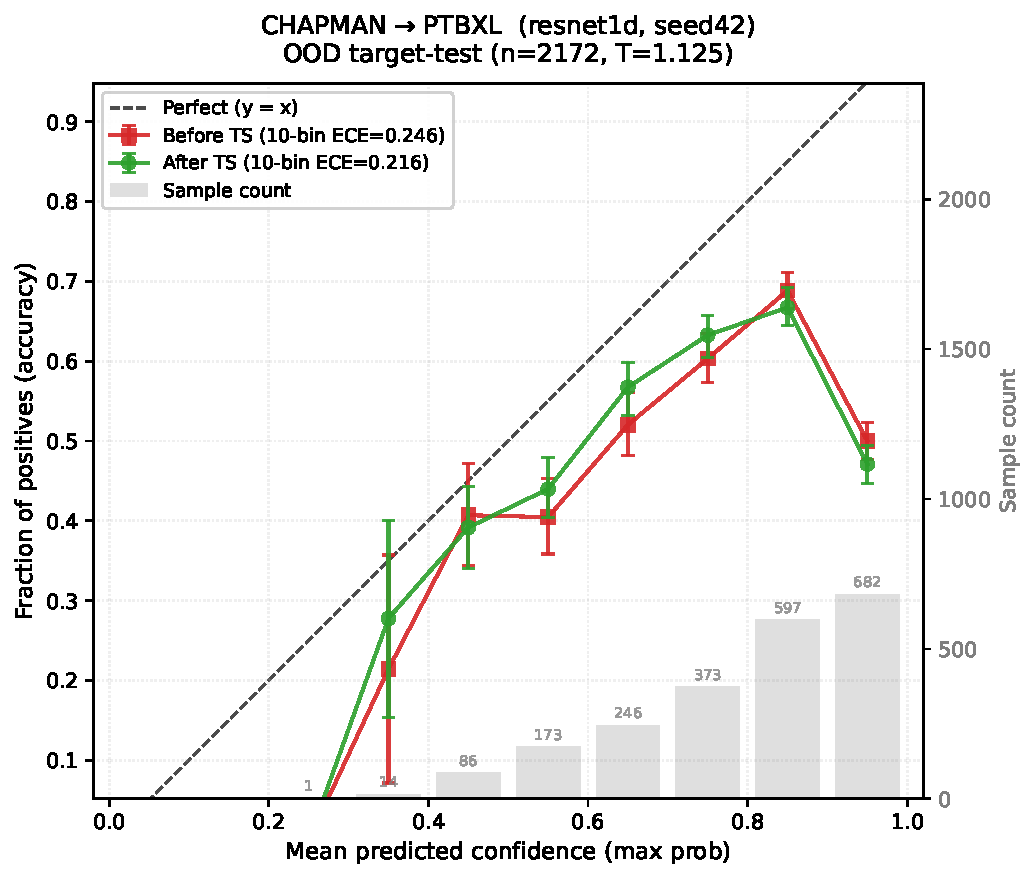
\includegraphics[width=0.32\textwidth]{figures/fig_reliability_supp_chapman_ptbxl_resnet1d_seed42.pdf}
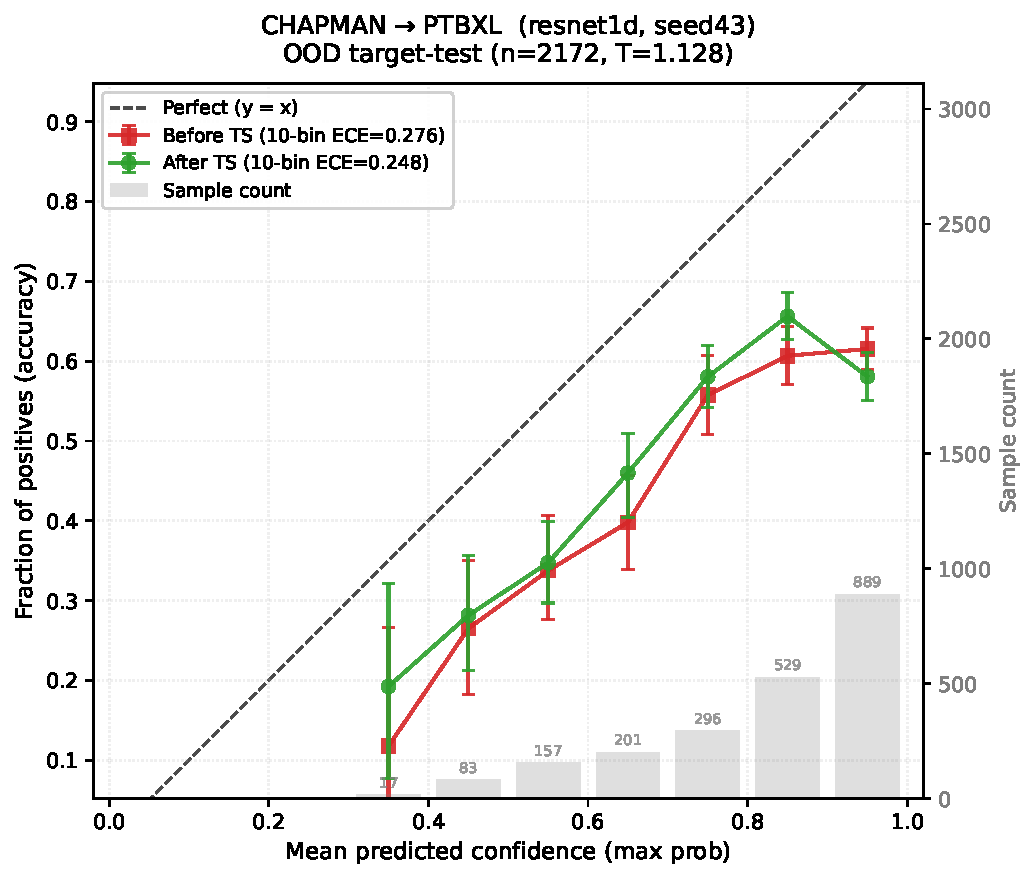
\includegraphics[width=0.32\textwidth]{figures/fig_reliability_supp_chapman_ptbxl_resnet1d_seed43.pdf}
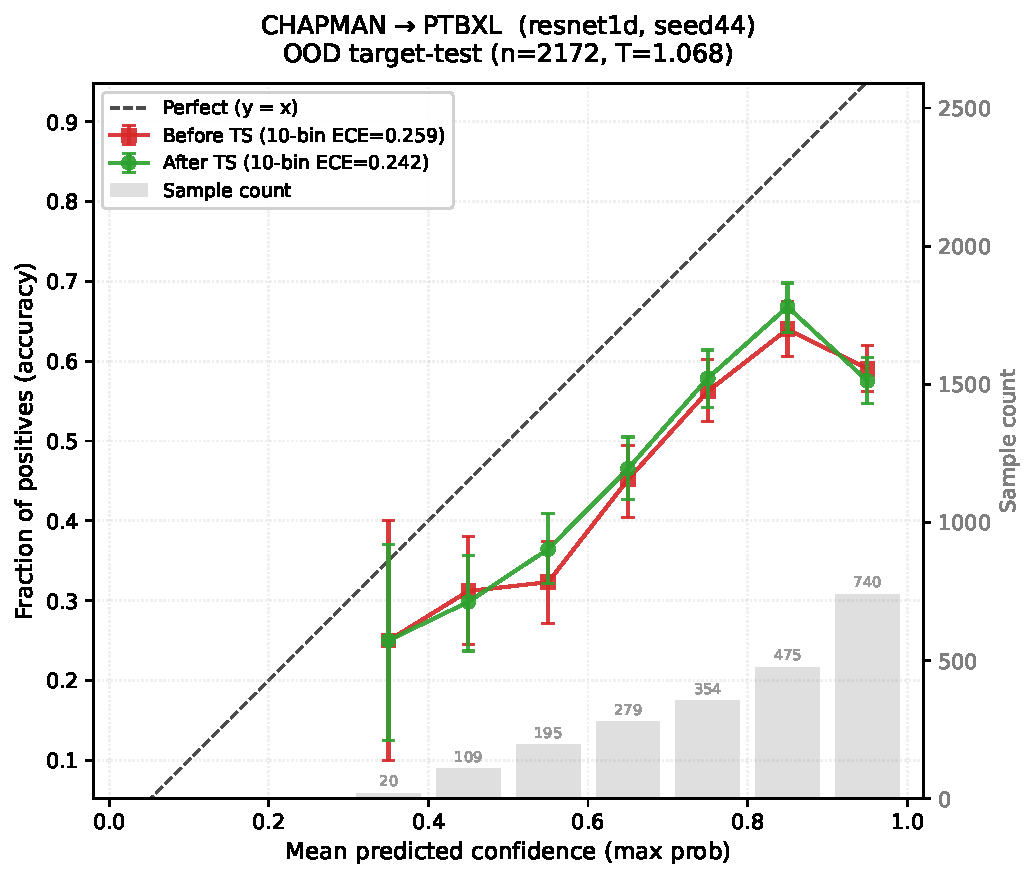
\includegraphics[width=0.32\textwidth]{figures/fig_reliability_supp_chapman_ptbxl_resnet1d_seed44.pdf}
\caption{Chapman$\to$PTB-XL 可靠性图：ResNet1D 种子 42--44。}
\end{figure}

\begin{figure}[h]
\centering
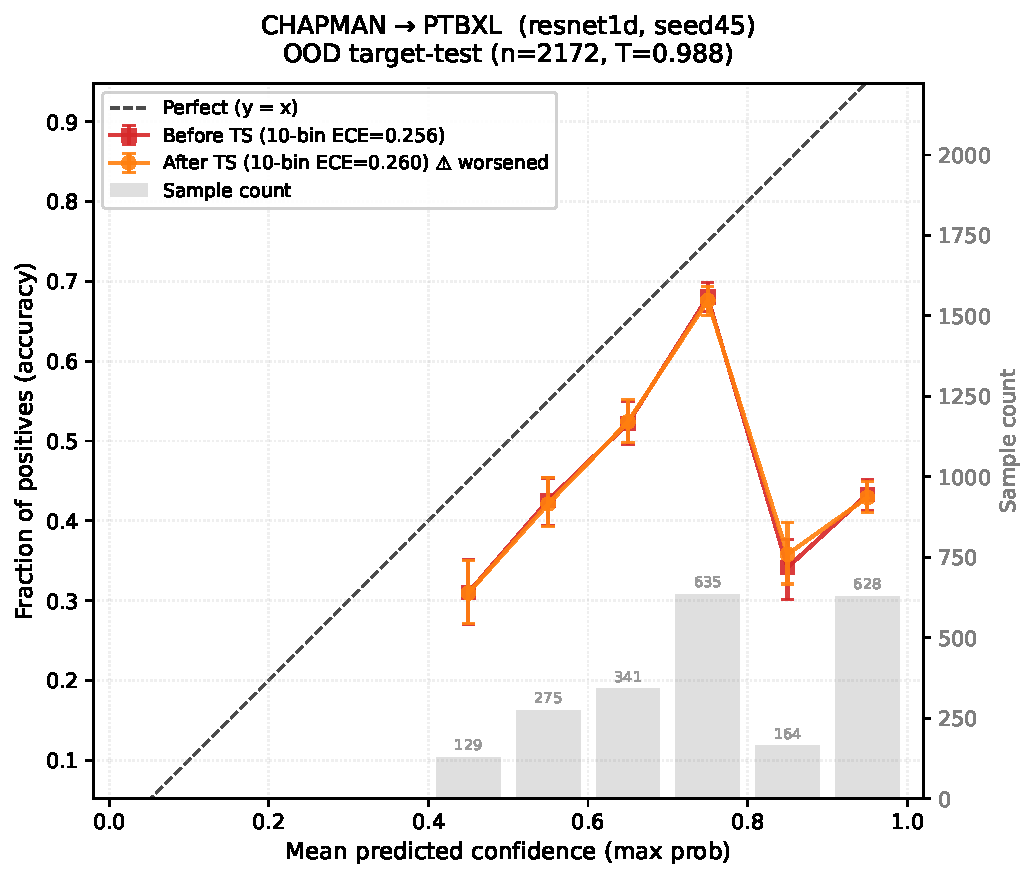
\includegraphics[width=0.45\textwidth]{figures/fig_reliability_supp_chapman_ptbxl_resnet1d_seed45.pdf}
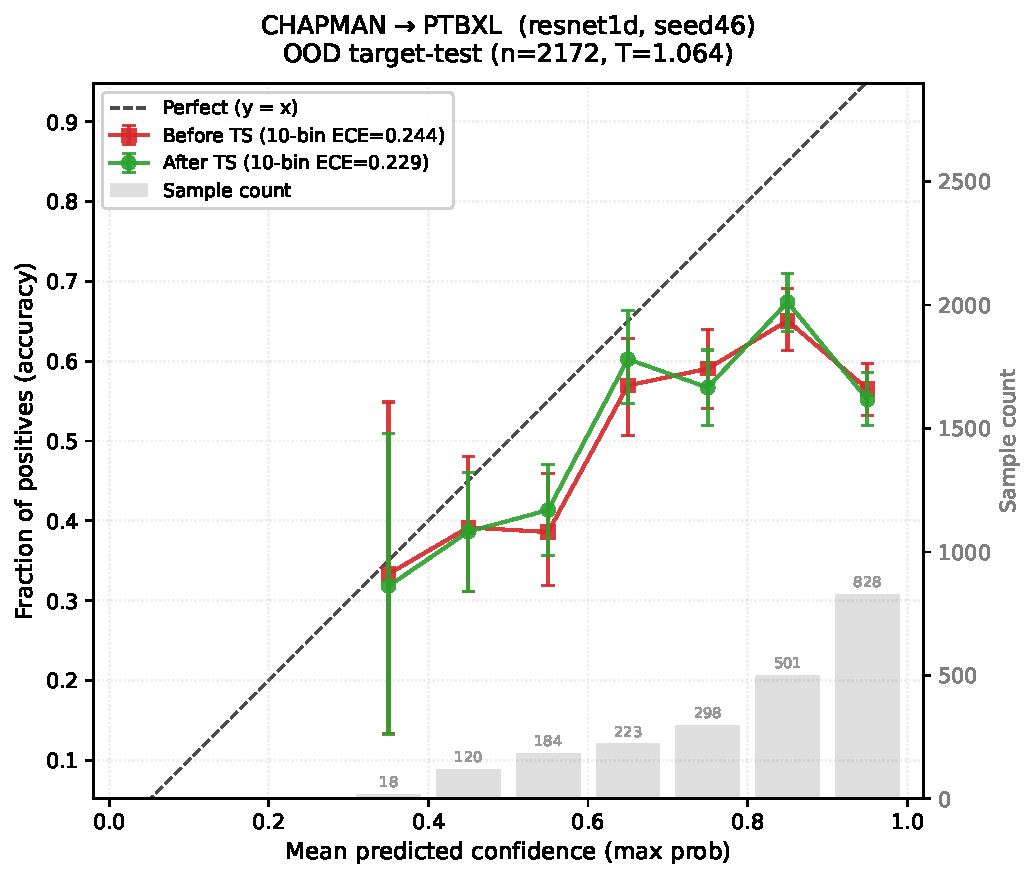
\includegraphics[width=0.45\textwidth]{figures/fig_reliability_supp_chapman_ptbxl_resnet1d_seed46.pdf}
\caption{Chapman$\to$PTB-XL 可靠性图：ResNet1D 种子 45--46。}
\end{figure}

\begin{figure}[h]
\centering
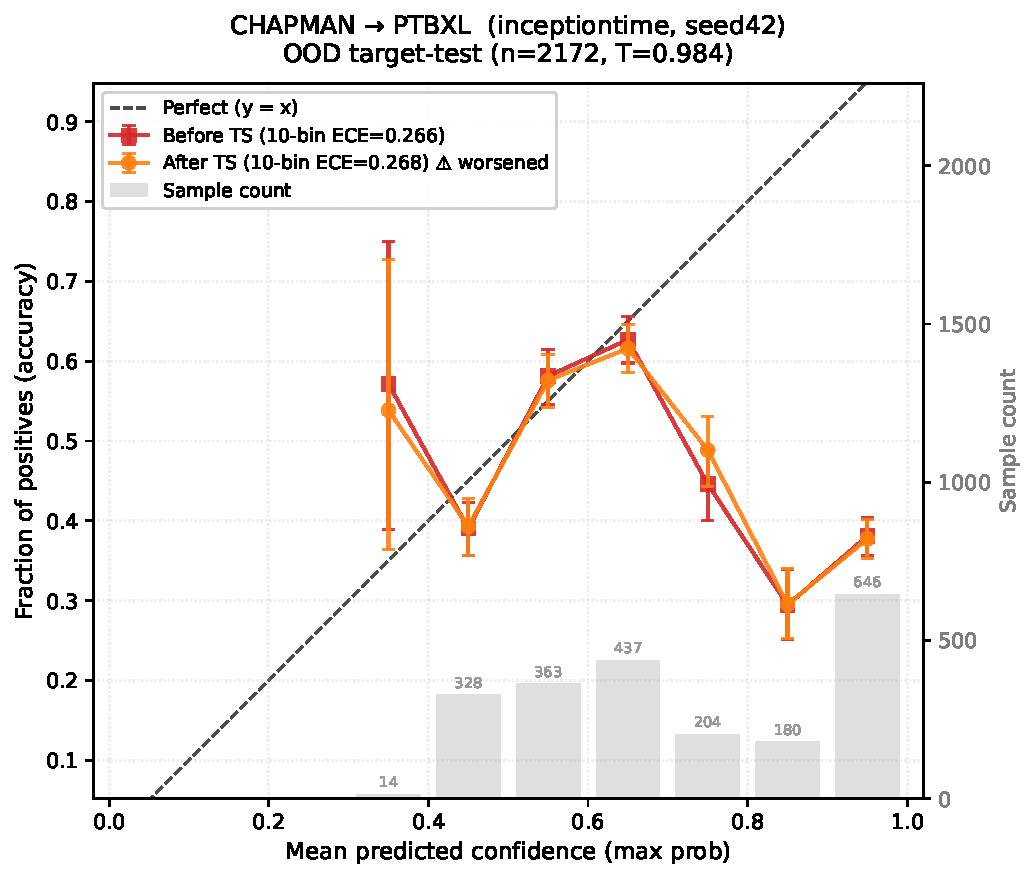
\includegraphics[width=0.32\textwidth]{figures/fig_reliability_supp_chapman_ptbxl_inceptiontime_seed42.pdf}
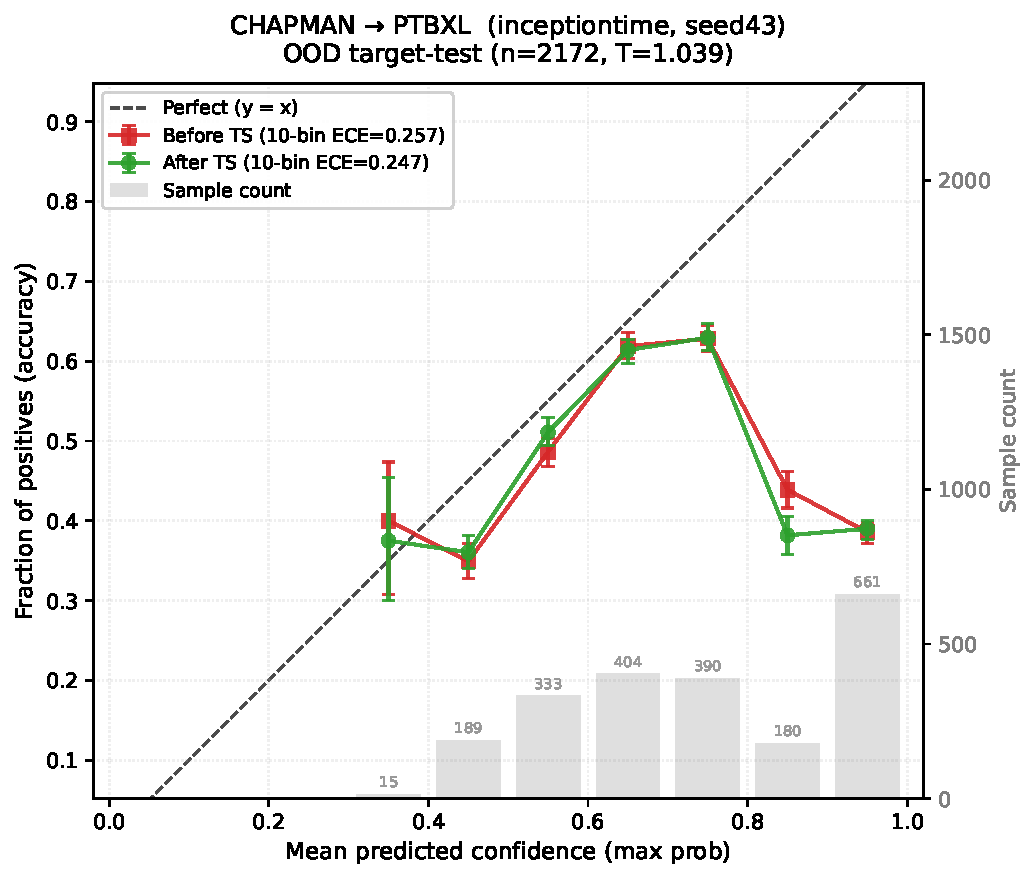
\includegraphics[width=0.32\textwidth]{figures/fig_reliability_supp_chapman_ptbxl_inceptiontime_seed43.pdf}
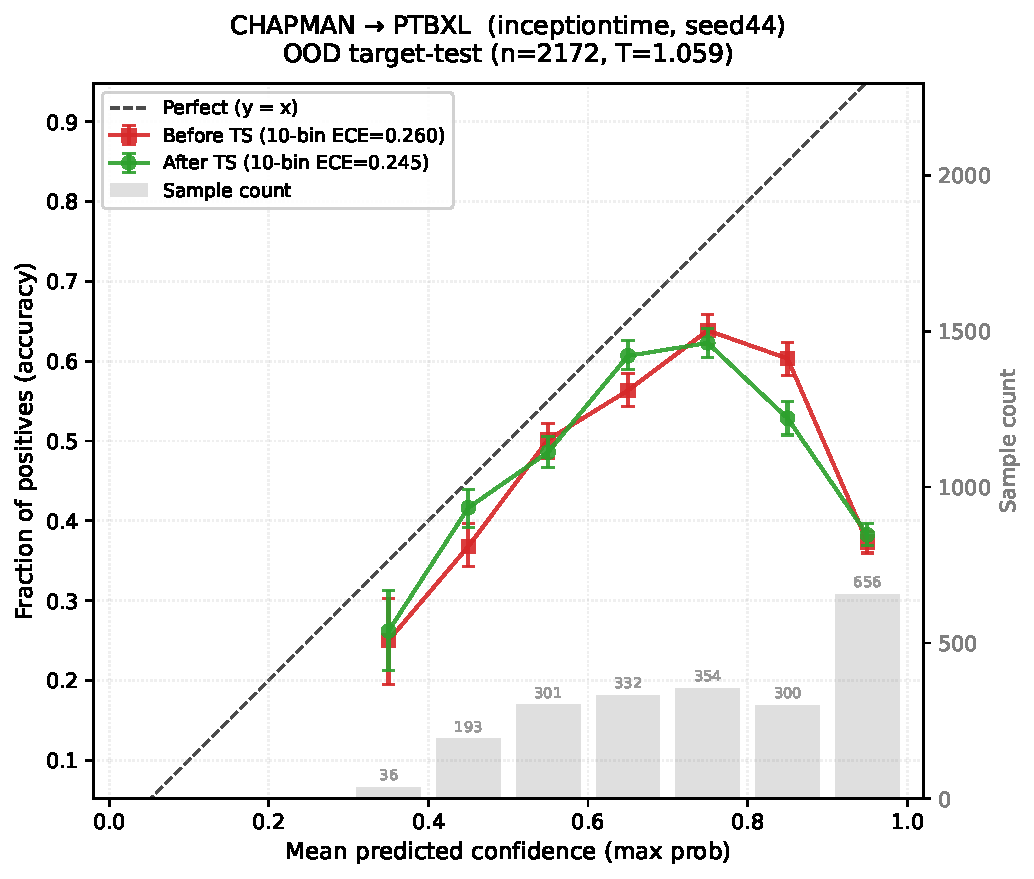
\includegraphics[width=0.32\textwidth]{figures/fig_reliability_supp_chapman_ptbxl_inceptiontime_seed44.pdf}
\caption{Chapman$\to$PTB-XL 可靠性图：InceptionTime 种子 42--44。}
\end{figure}

\begin{figure}[h]
\centering
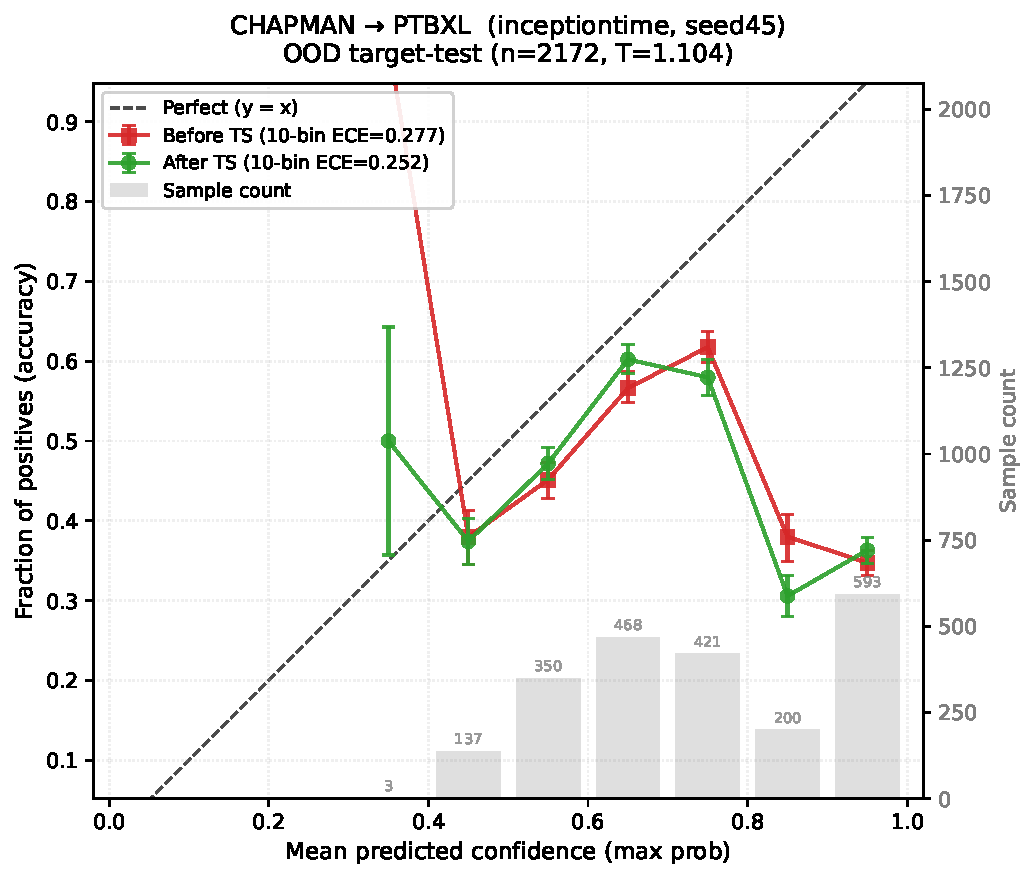
\includegraphics[width=0.45\textwidth]{figures/fig_reliability_supp_chapman_ptbxl_inceptiontime_seed45.pdf}
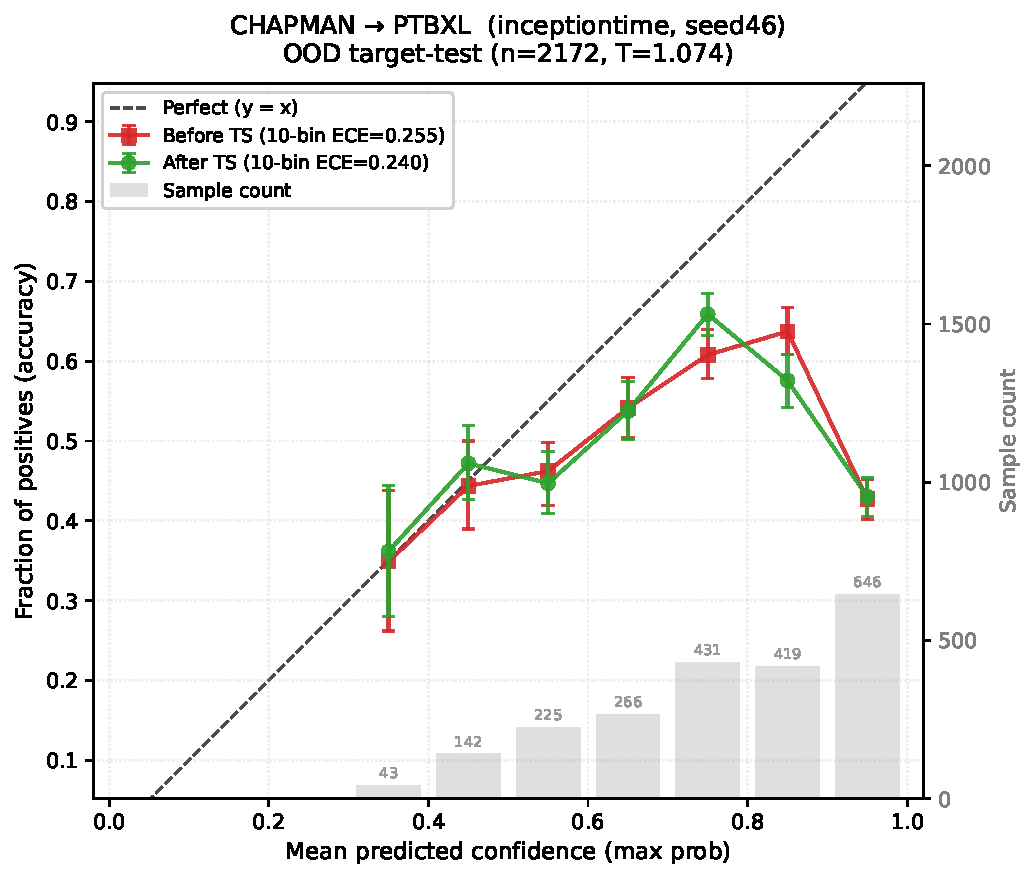
\includegraphics[width=0.45\textwidth]{figures/fig_reliability_supp_chapman_ptbxl_inceptiontime_seed46.pdf}
\caption{Chapman$\to$PTB-XL 可靠性图：InceptionTime 种子 45--46。}
\end{figure}

\subsubsection*{S1.3.\ CPSC$\rightarrow$Chapman}

\begin{figure}[h]
\centering
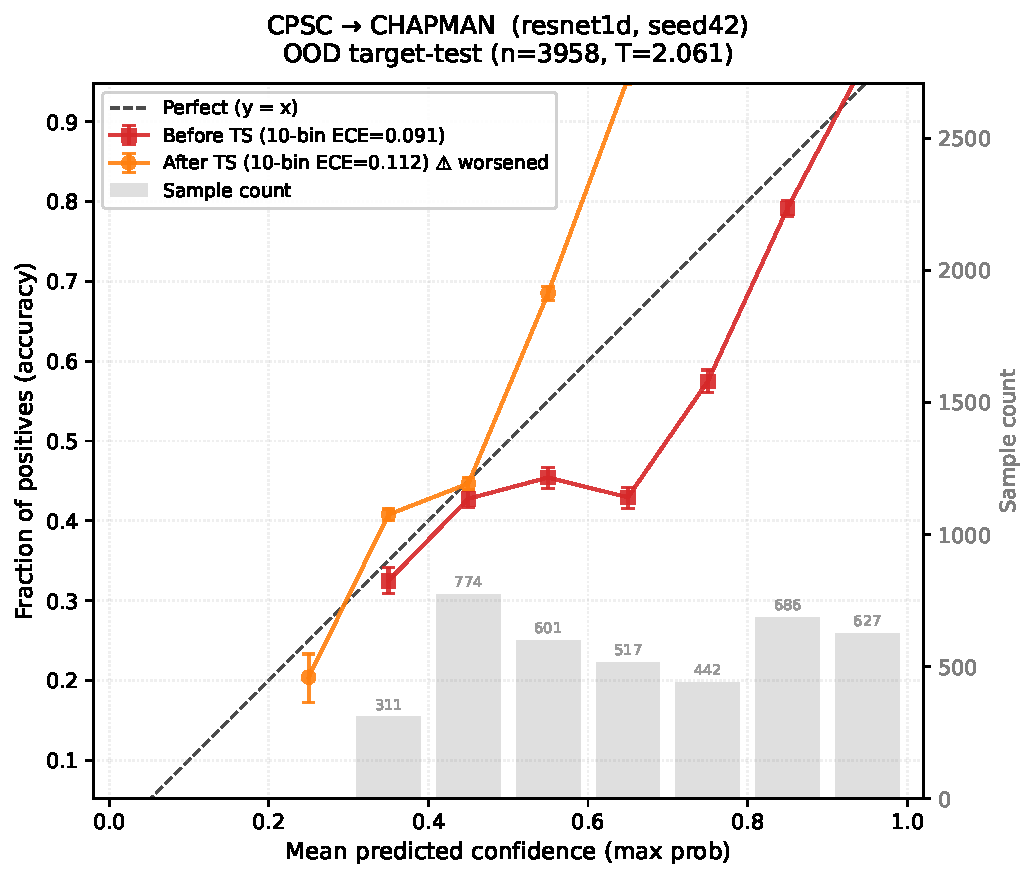
\includegraphics[width=0.32\textwidth]{figures/fig_reliability_supp_cpsc_chapman_resnet1d_seed42.pdf}
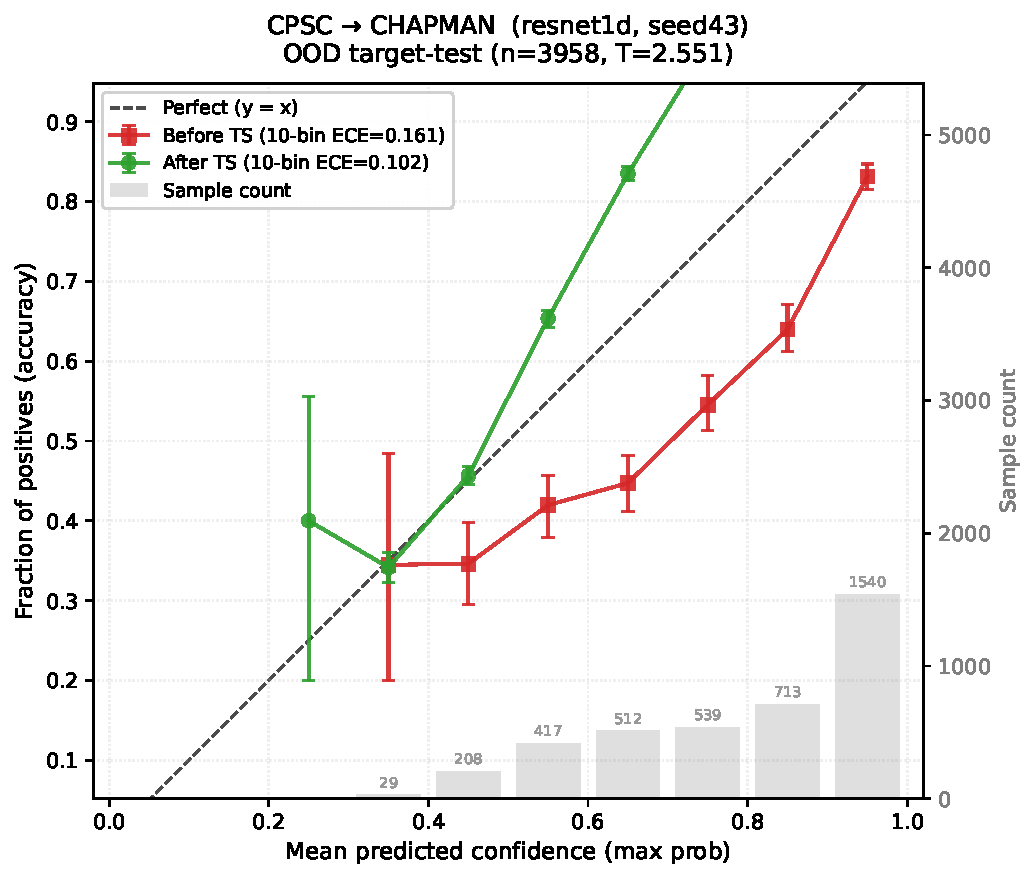
\includegraphics[width=0.32\textwidth]{figures/fig_reliability_supp_cpsc_chapman_resnet1d_seed43.pdf}
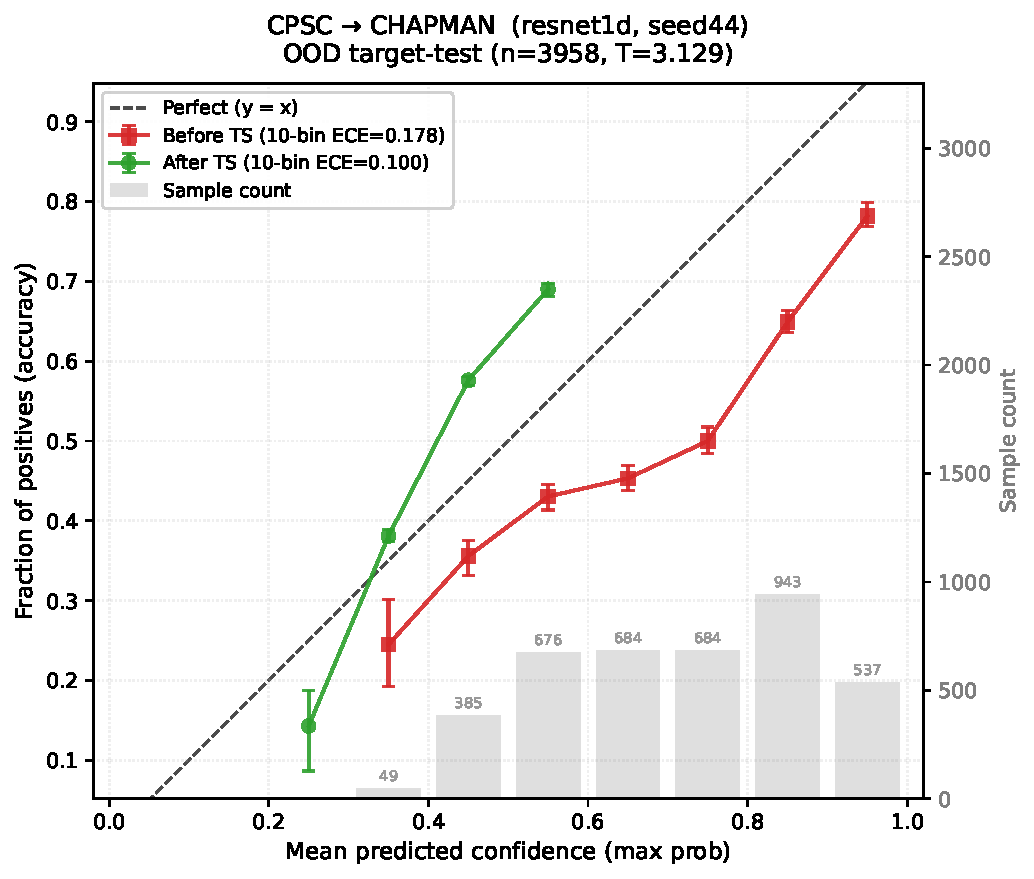
\includegraphics[width=0.32\textwidth]{figures/fig_reliability_supp_cpsc_chapman_resnet1d_seed44.pdf}
\caption{CPSC$\to$Chapman 可靠性图：ResNet1D 种子 42--44。}
\end{figure}

\begin{figure}[h]
\centering
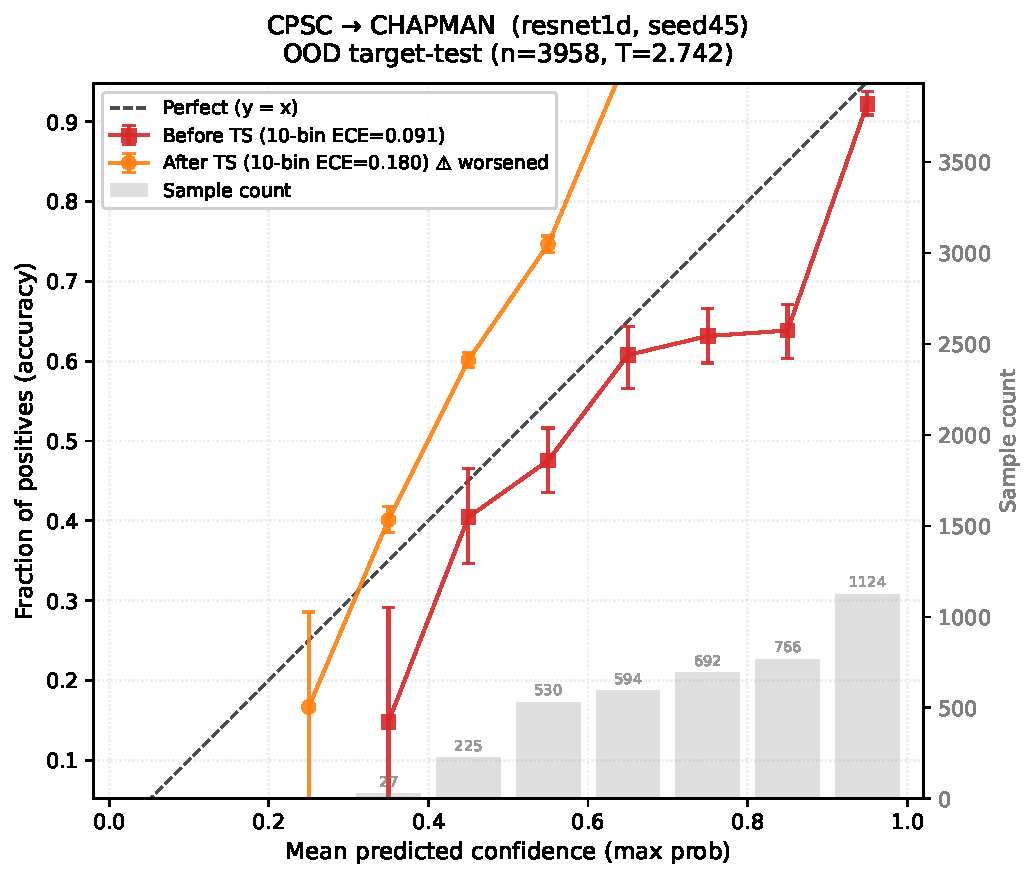
\includegraphics[width=0.45\textwidth]{figures/fig_reliability_supp_cpsc_chapman_resnet1d_seed45.pdf}
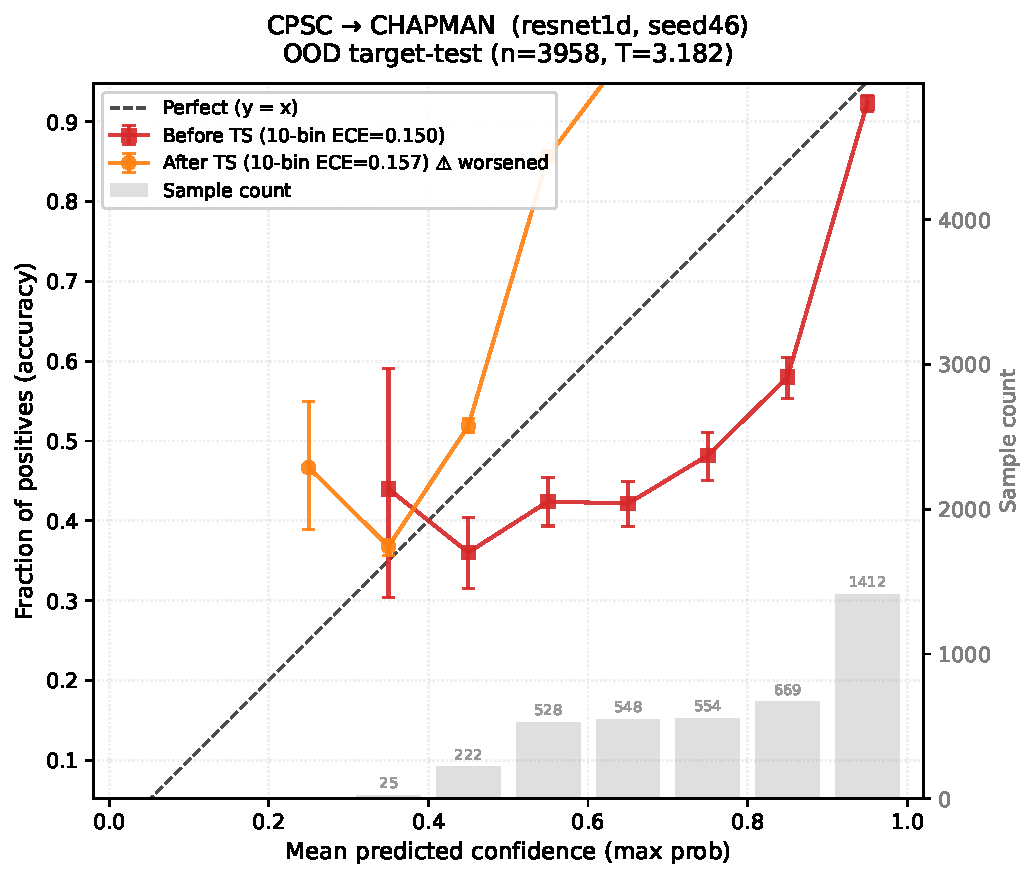
\includegraphics[width=0.45\textwidth]{figures/fig_reliability_supp_cpsc_chapman_resnet1d_seed46.pdf}
\caption{CPSC$\to$Chapman 可靠性图：ResNet1D 种子 45--46。}
\end{figure}

\begin{figure}[h]
\centering
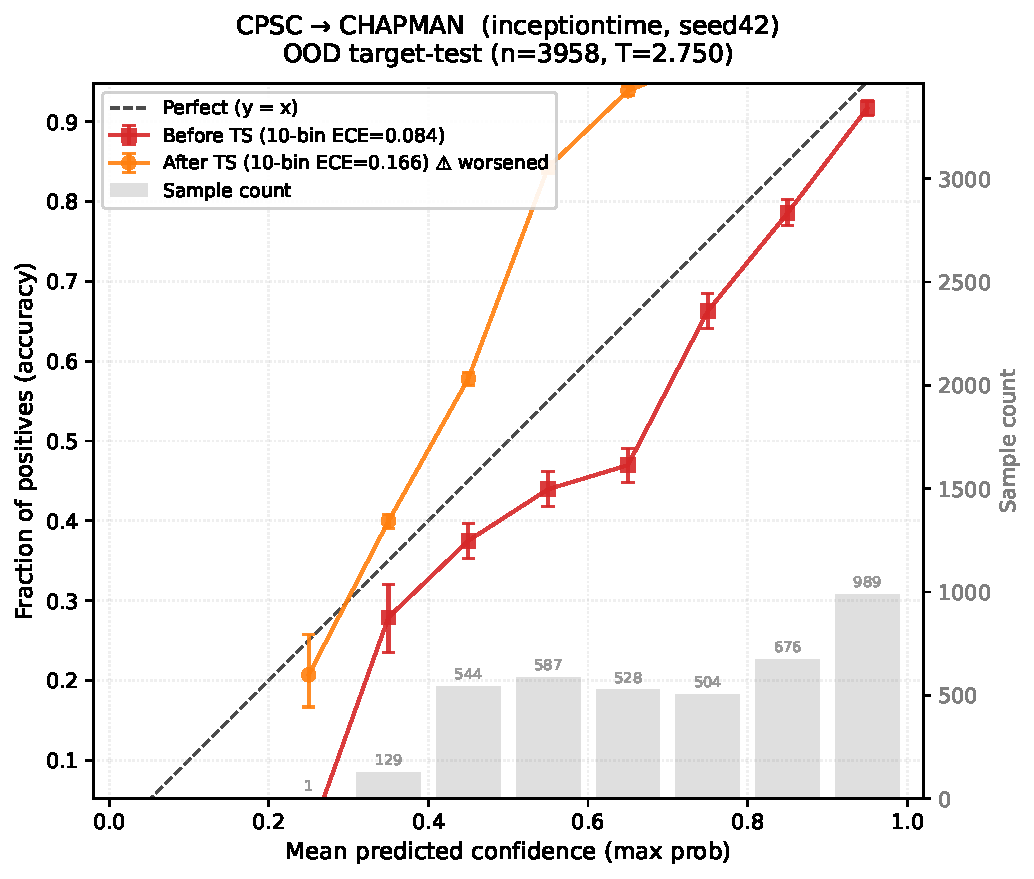
\includegraphics[width=0.32\textwidth]{figures/fig_reliability_supp_cpsc_chapman_inceptiontime_seed42.pdf}
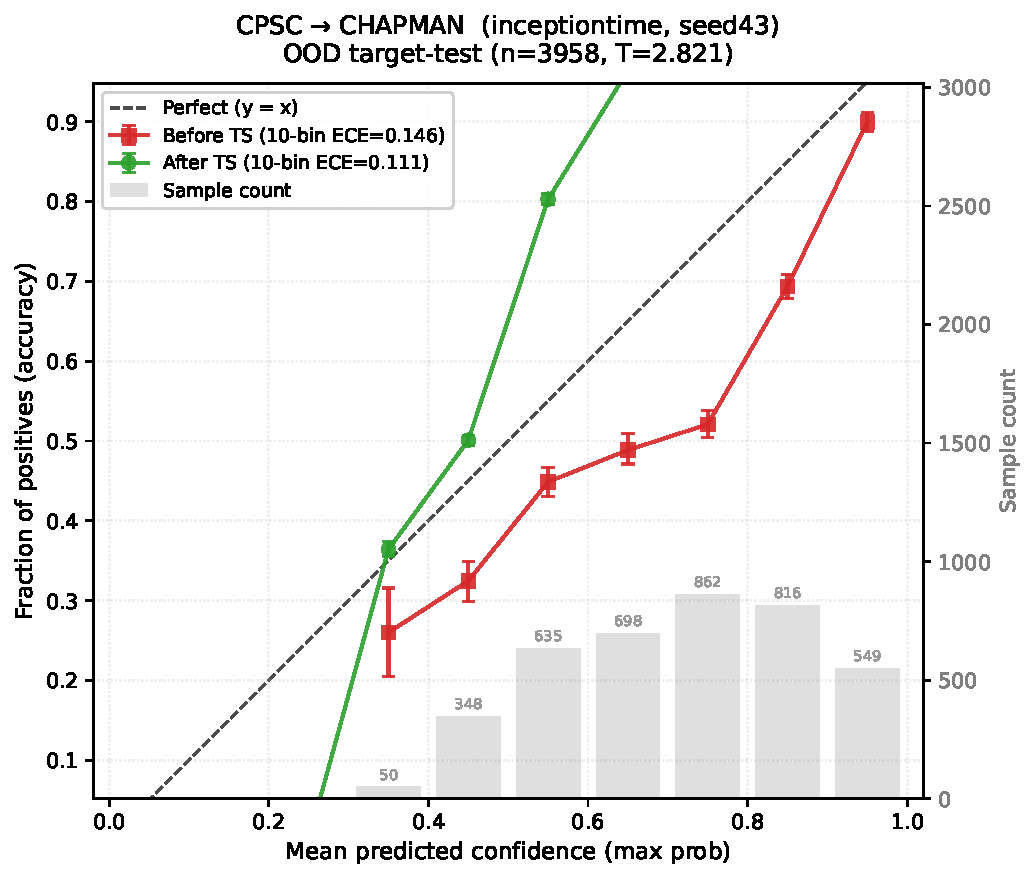
\includegraphics[width=0.32\textwidth]{figures/fig_reliability_supp_cpsc_chapman_inceptiontime_seed43.pdf}
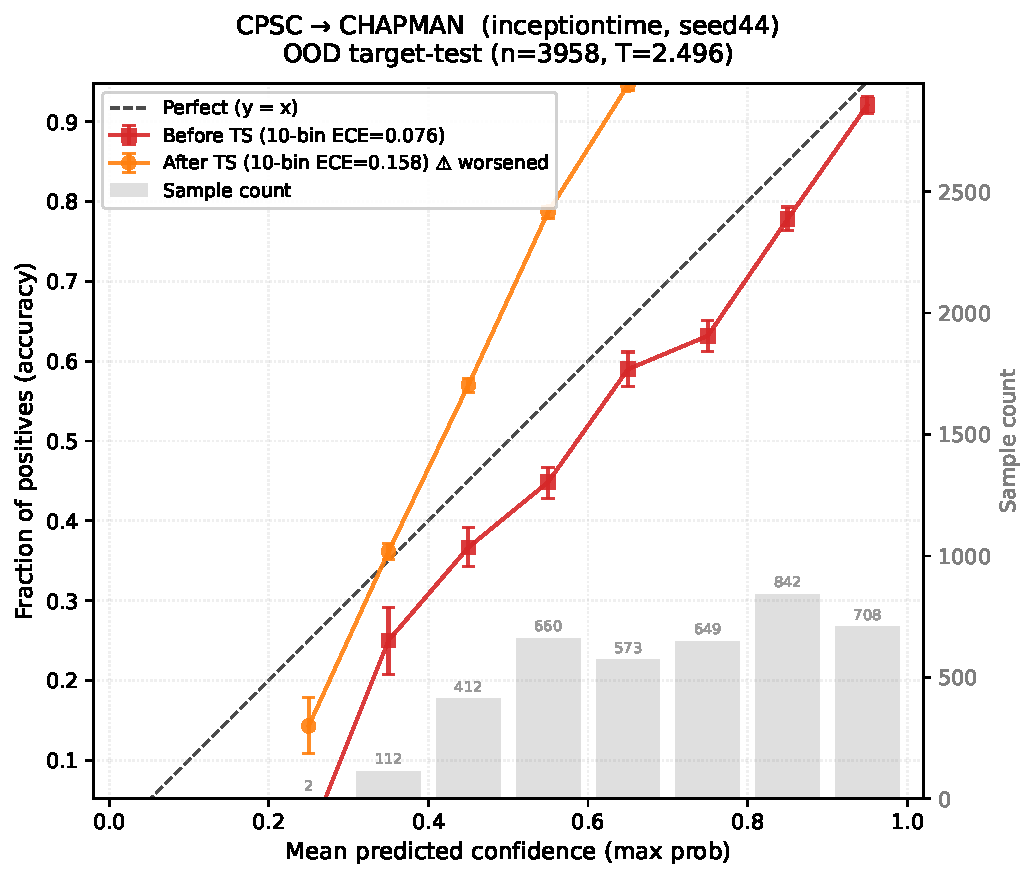
\includegraphics[width=0.32\textwidth]{figures/fig_reliability_supp_cpsc_chapman_inceptiontime_seed44.pdf}
\caption{CPSC$\to$Chapman 可靠性图：InceptionTime 种子 42--44。}
\end{figure}

\begin{figure}[h]
\centering
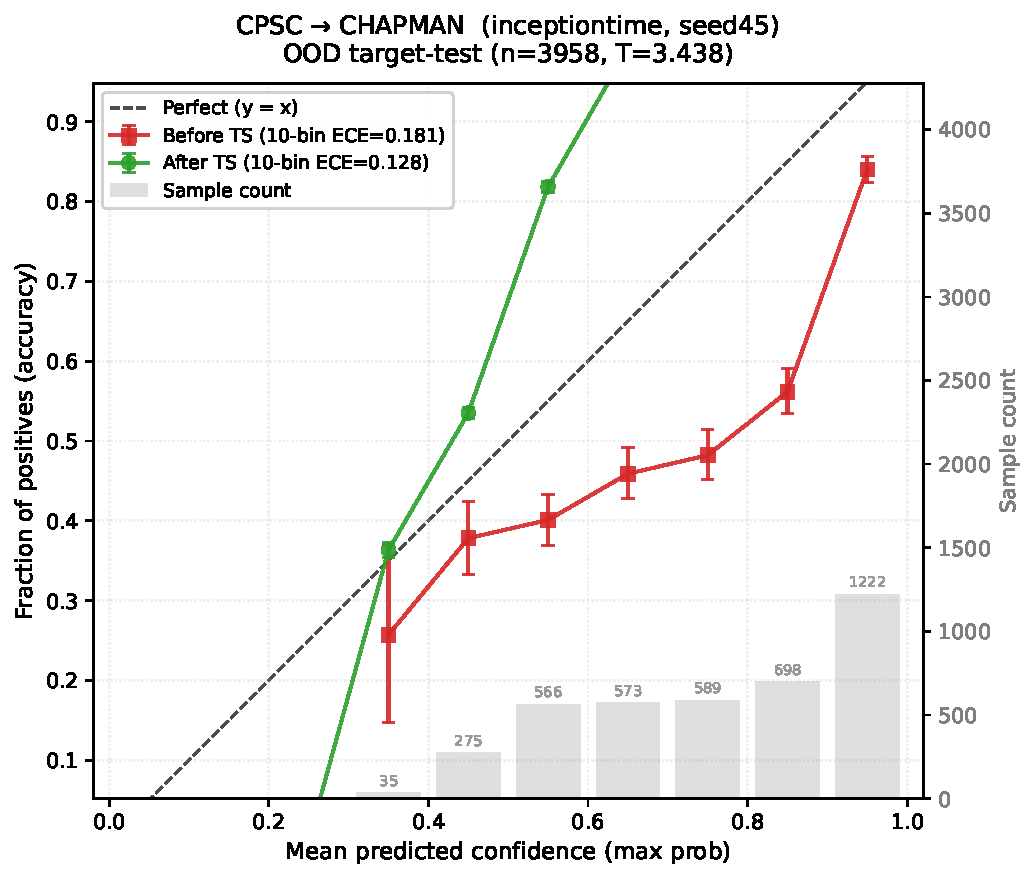
\includegraphics[width=0.45\textwidth]{figures/fig_reliability_supp_cpsc_chapman_inceptiontime_seed45.pdf}
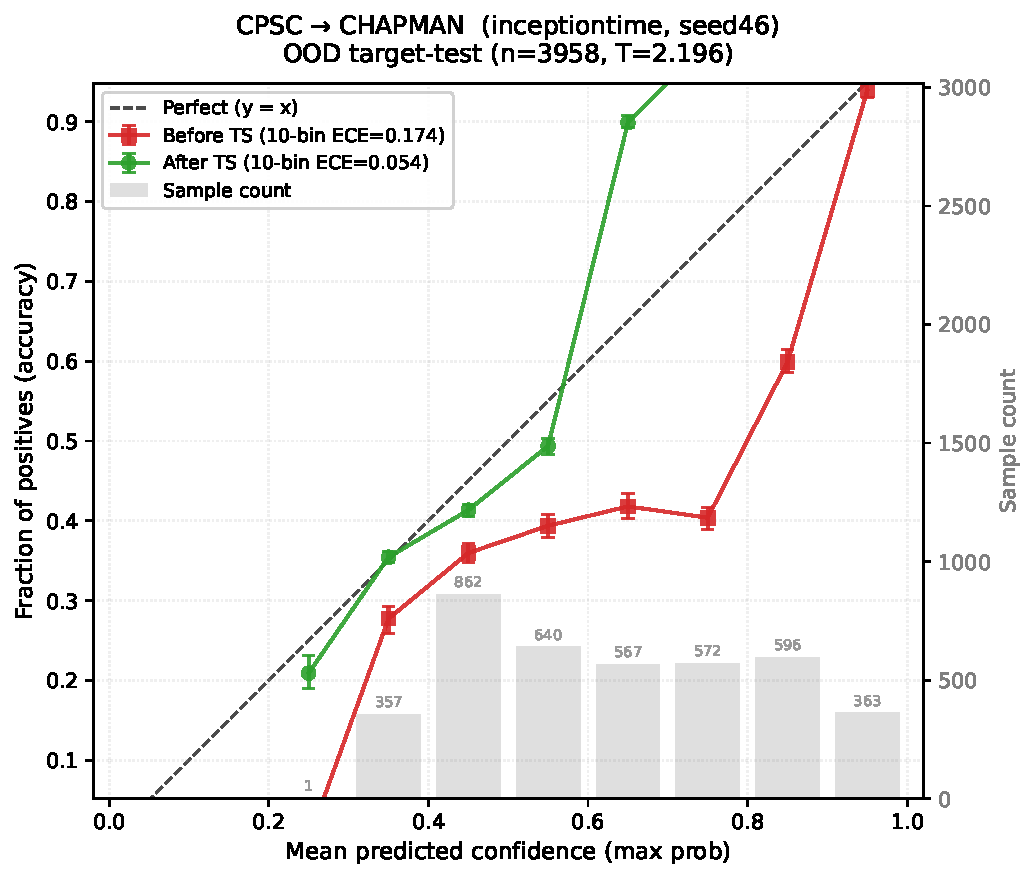
\includegraphics[width=0.45\textwidth]{figures/fig_reliability_supp_cpsc_chapman_inceptiontime_seed46.pdf}
\caption{CPSC$\to$Chapman 可靠性图：InceptionTime 种子 45--46。}
\end{figure}

\subsubsection*{S1.4.\ CPSC$\rightarrow$PTB-XL}

\begin{figure}[h]
\centering
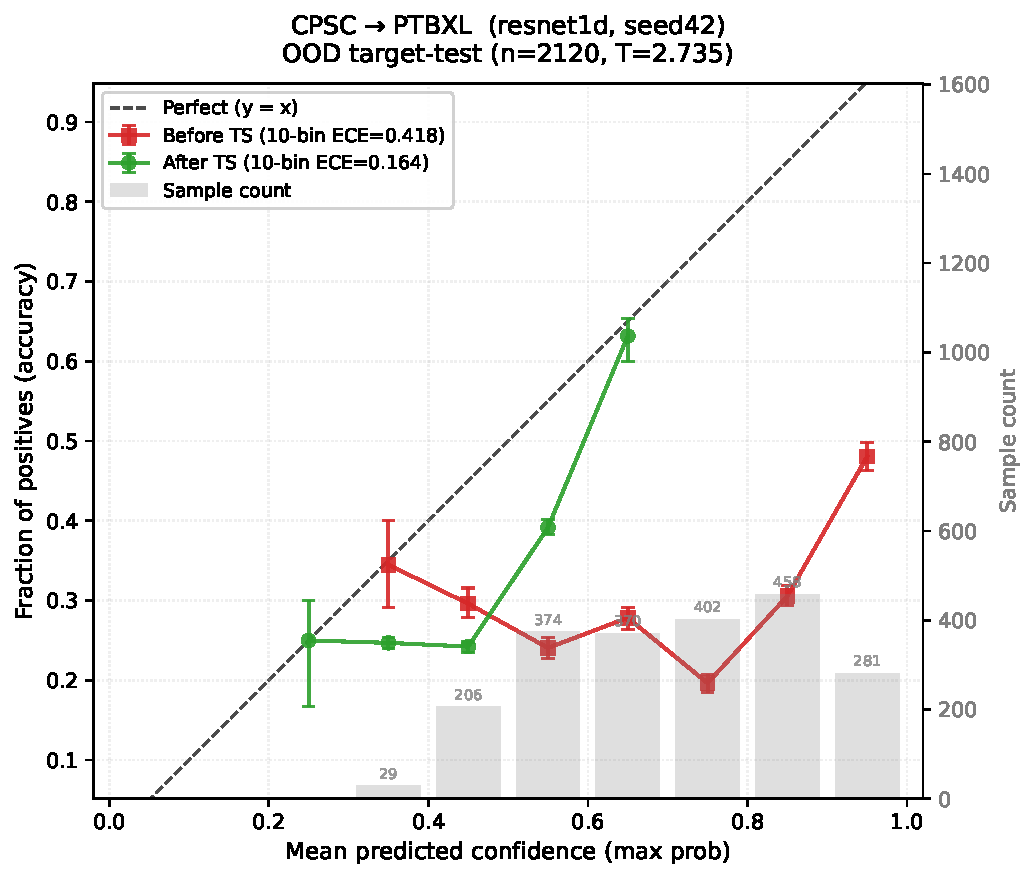
\includegraphics[width=0.32\textwidth]{figures/fig_reliability_supp_cpsc_ptbxl_resnet1d_seed42.pdf}
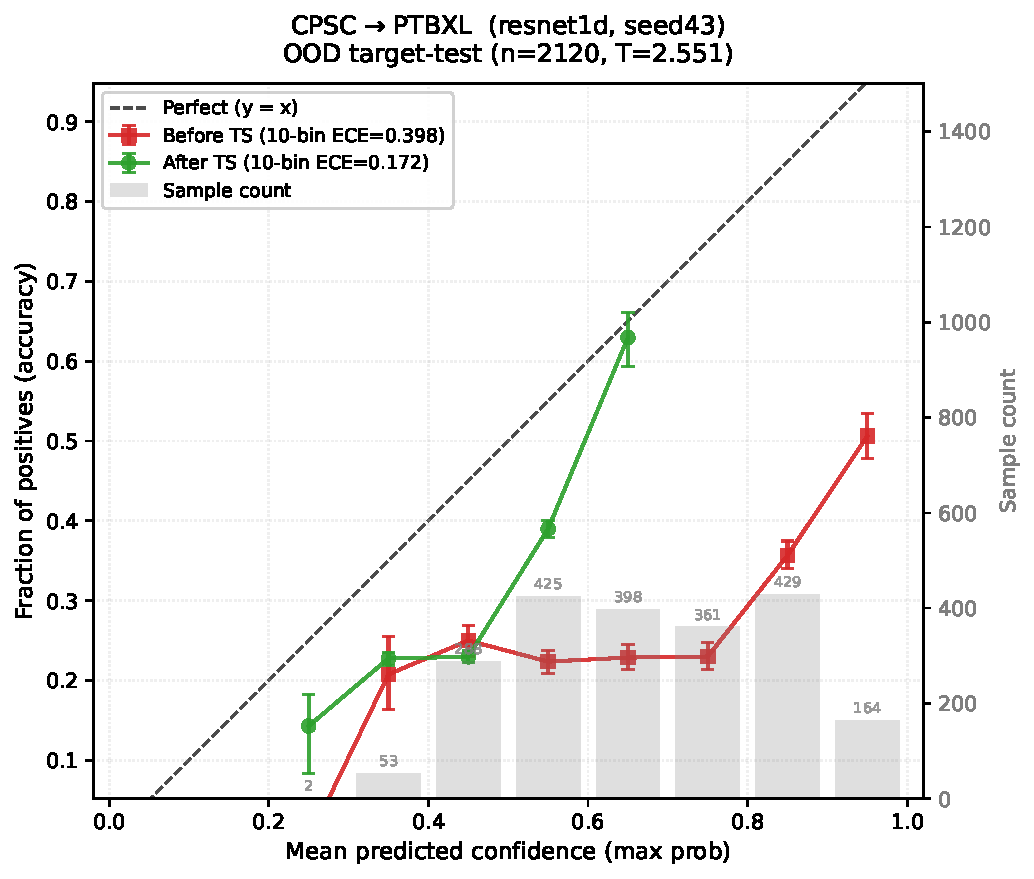
\includegraphics[width=0.32\textwidth]{figures/fig_reliability_supp_cpsc_ptbxl_resnet1d_seed43.pdf}
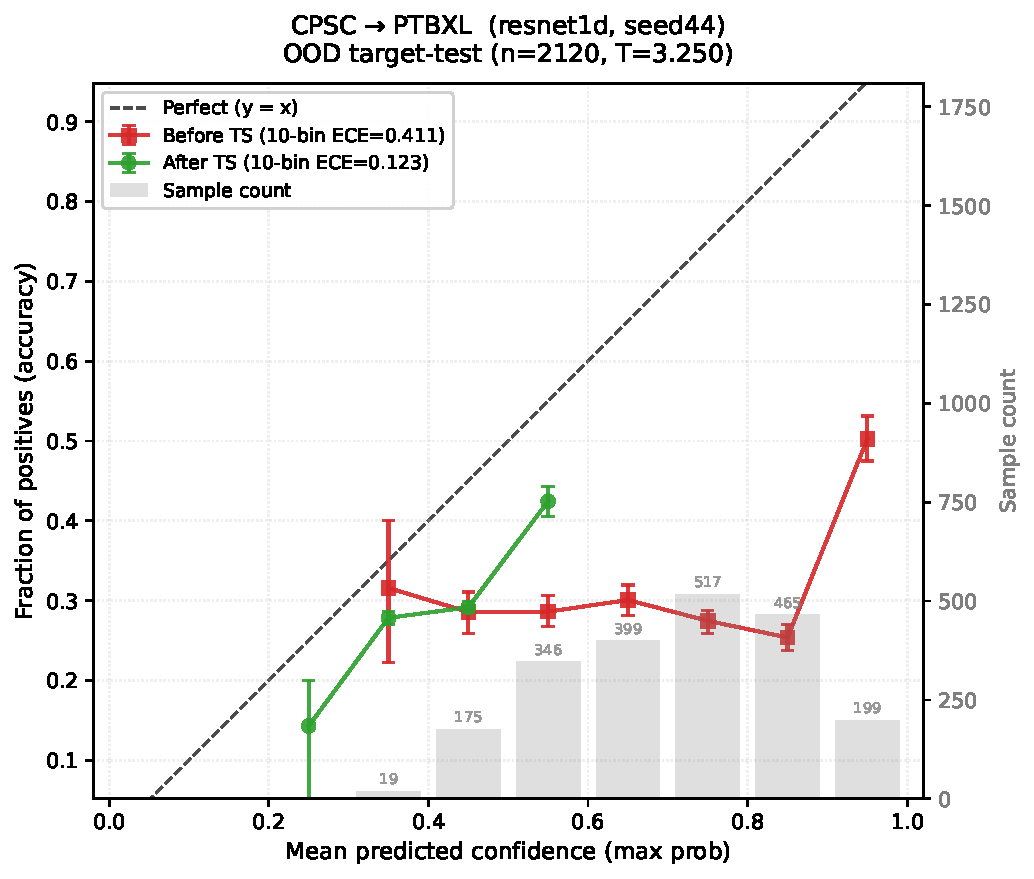
\includegraphics[width=0.32\textwidth]{figures/fig_reliability_supp_cpsc_ptbxl_resnet1d_seed44.pdf}
\caption{CPSC$\to$PTB-XL 可靠性图：ResNet1D 种子 42--44。}
\end{figure}

\begin{figure}[h]
\centering
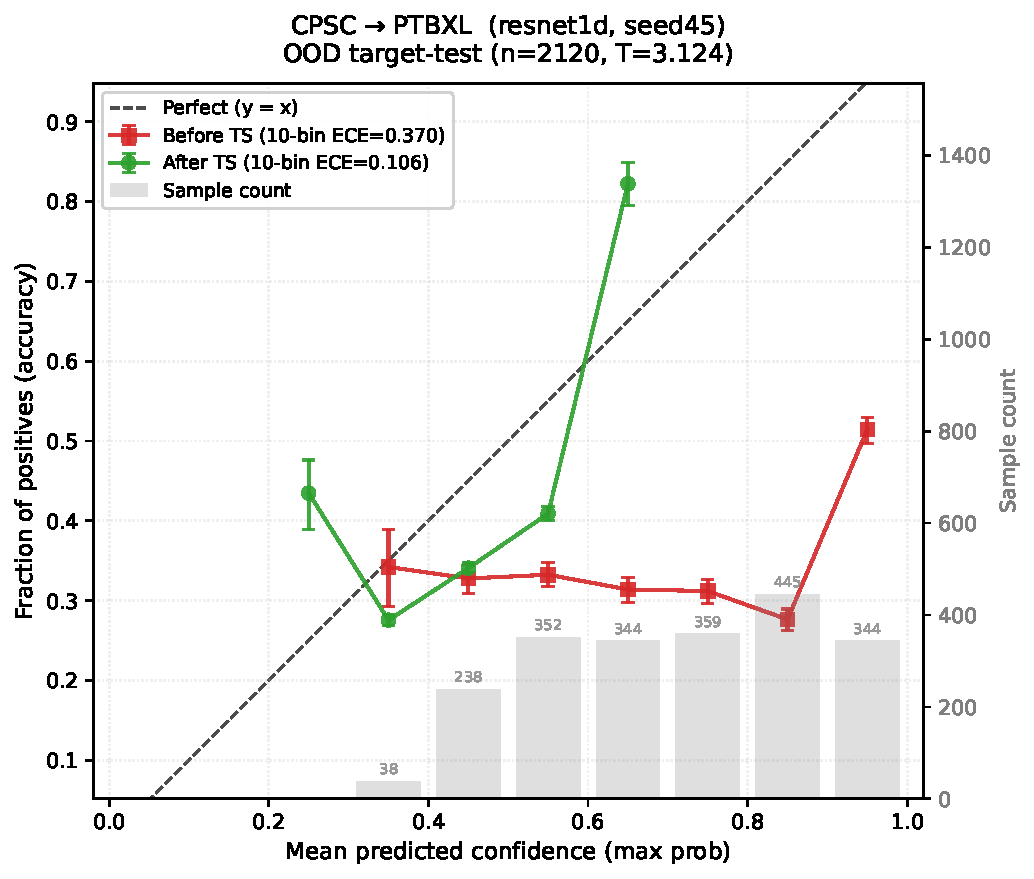
\includegraphics[width=0.45\textwidth]{figures/fig_reliability_supp_cpsc_ptbxl_resnet1d_seed45.pdf}
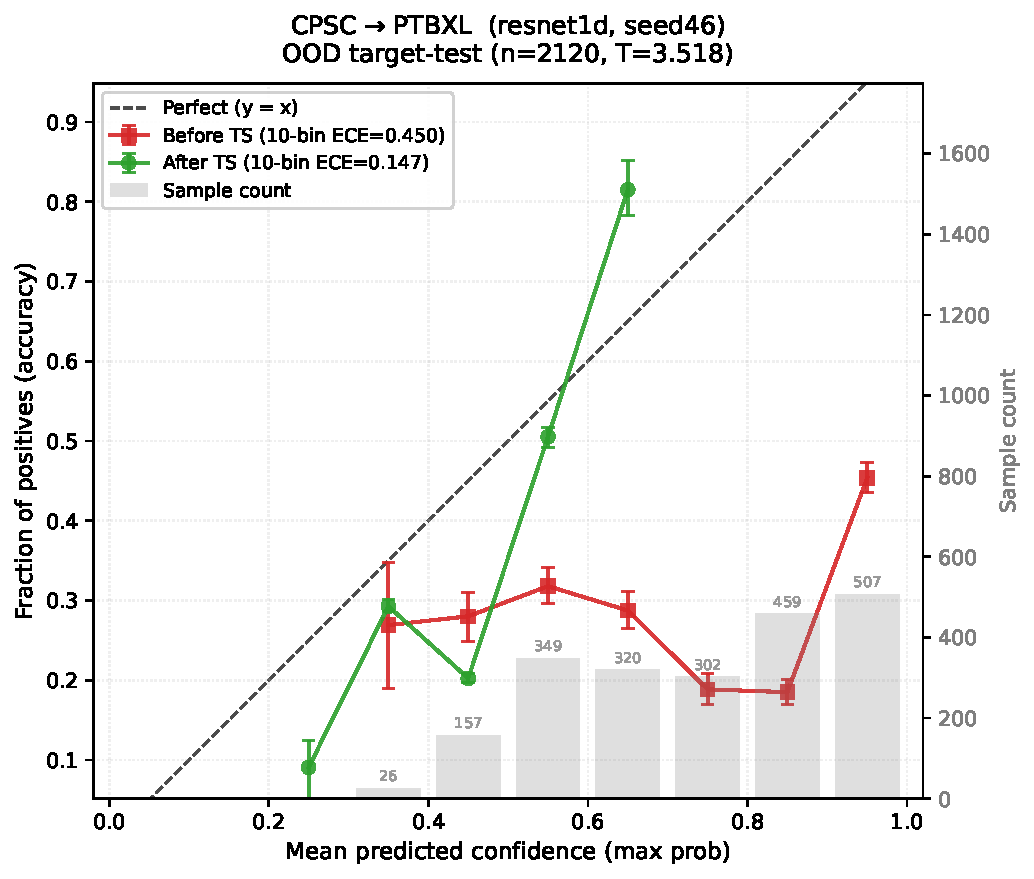
\includegraphics[width=0.45\textwidth]{figures/fig_reliability_supp_cpsc_ptbxl_resnet1d_seed46.pdf}
\caption{CPSC$\to$PTB-XL 可靠性图：ResNet1D 种子 45--46。}
\end{figure}

\begin{figure}[h]
\centering
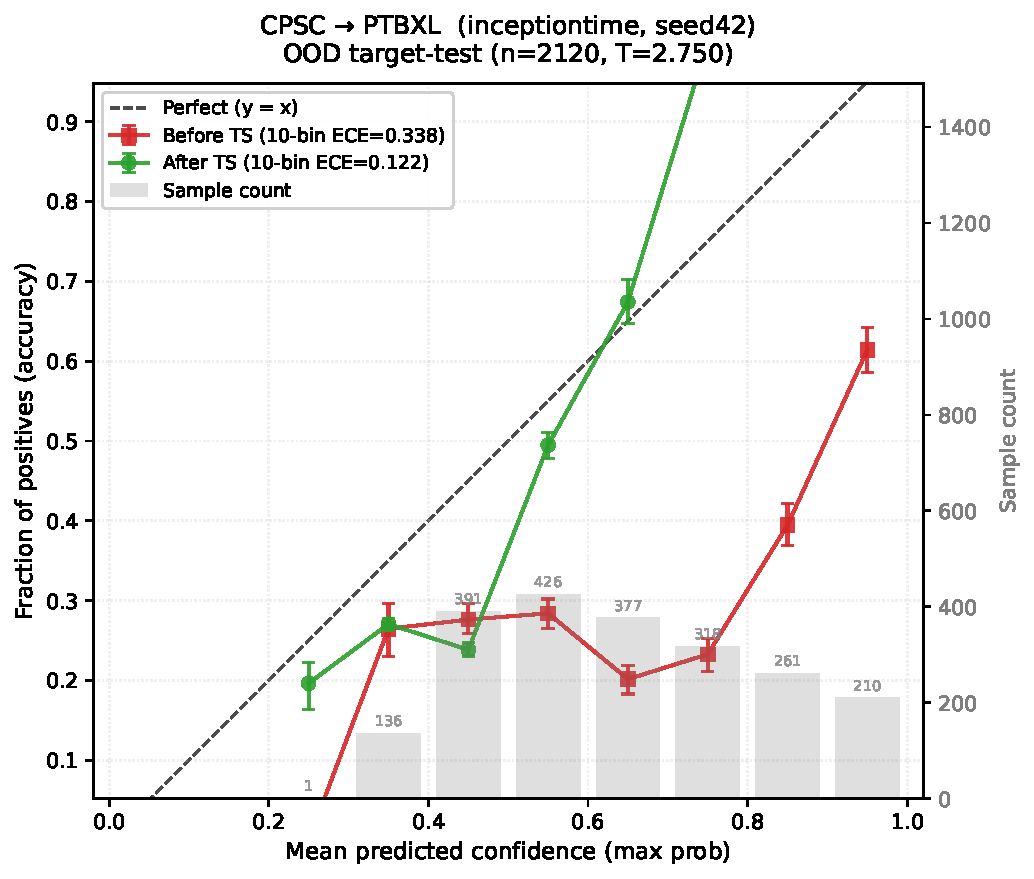
\includegraphics[width=0.32\textwidth]{figures/fig_reliability_supp_cpsc_ptbxl_inceptiontime_seed42.pdf}
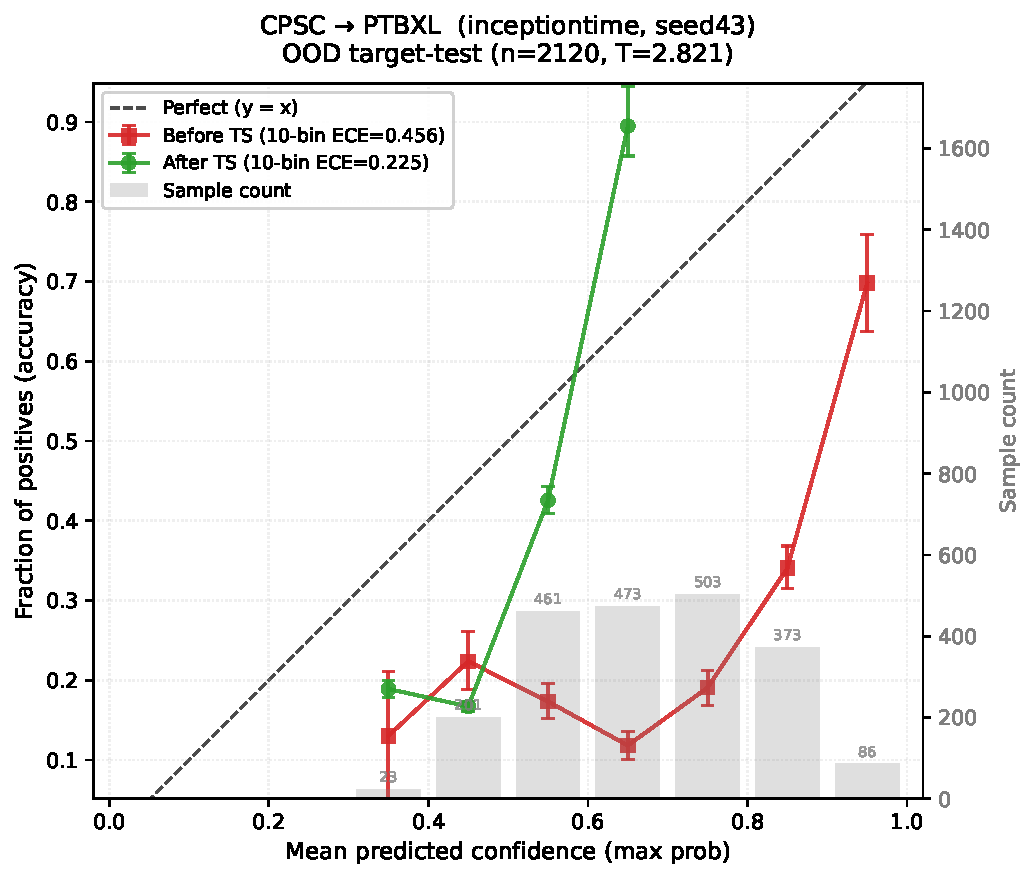
\includegraphics[width=0.32\textwidth]{figures/fig_reliability_supp_cpsc_ptbxl_inceptiontime_seed43.pdf}
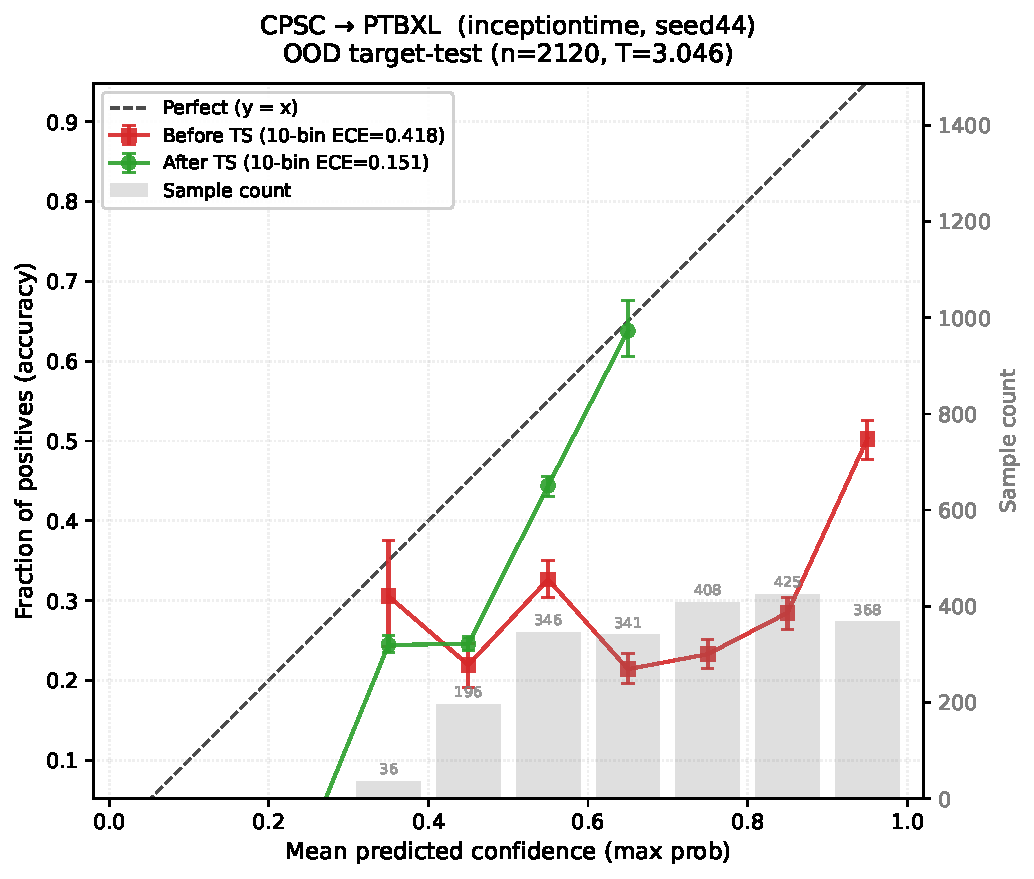
\includegraphics[width=0.32\textwidth]{figures/fig_reliability_supp_cpsc_ptbxl_inceptiontime_seed44.pdf}
\caption{CPSC$\to$PTB-XL 可靠性图：InceptionTime 种子 42--44。}
\end{figure}

\begin{figure}[h]
\centering
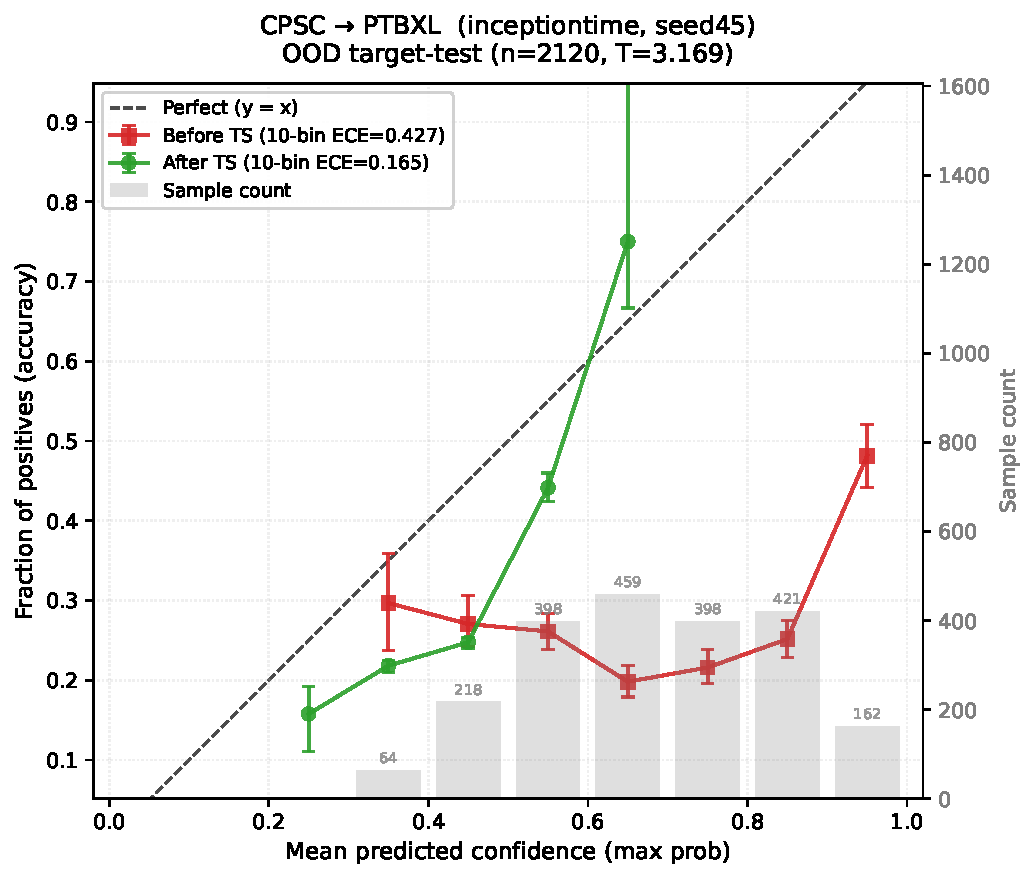
\includegraphics[width=0.45\textwidth]{figures/fig_reliability_supp_cpsc_ptbxl_inceptiontime_seed45.pdf}
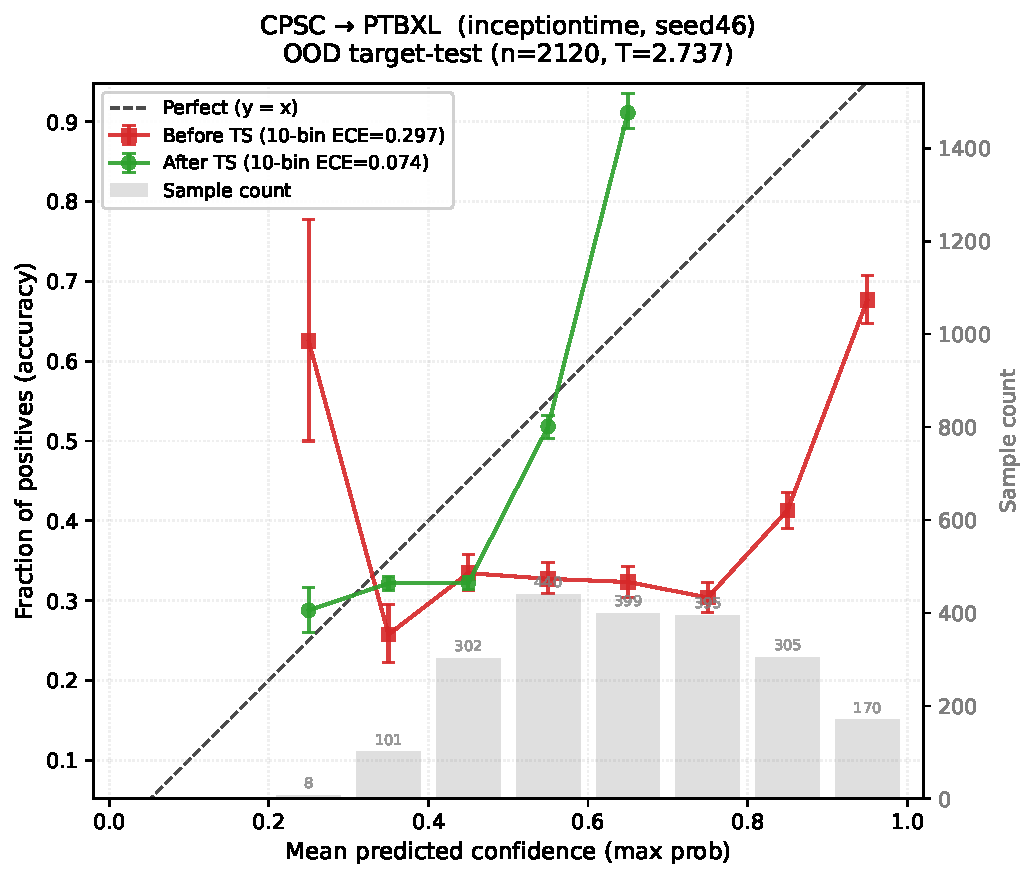
\includegraphics[width=0.45\textwidth]{figures/fig_reliability_supp_cpsc_ptbxl_inceptiontime_seed46.pdf}
\caption{CPSC$\to$PTB-XL 可靠性图：InceptionTime 种子 45--46。}
\end{figure}

\subsubsection*{S1.5.\ PTB-XL$\rightarrow$Chapman}

\begin{figure}[h]
\centering
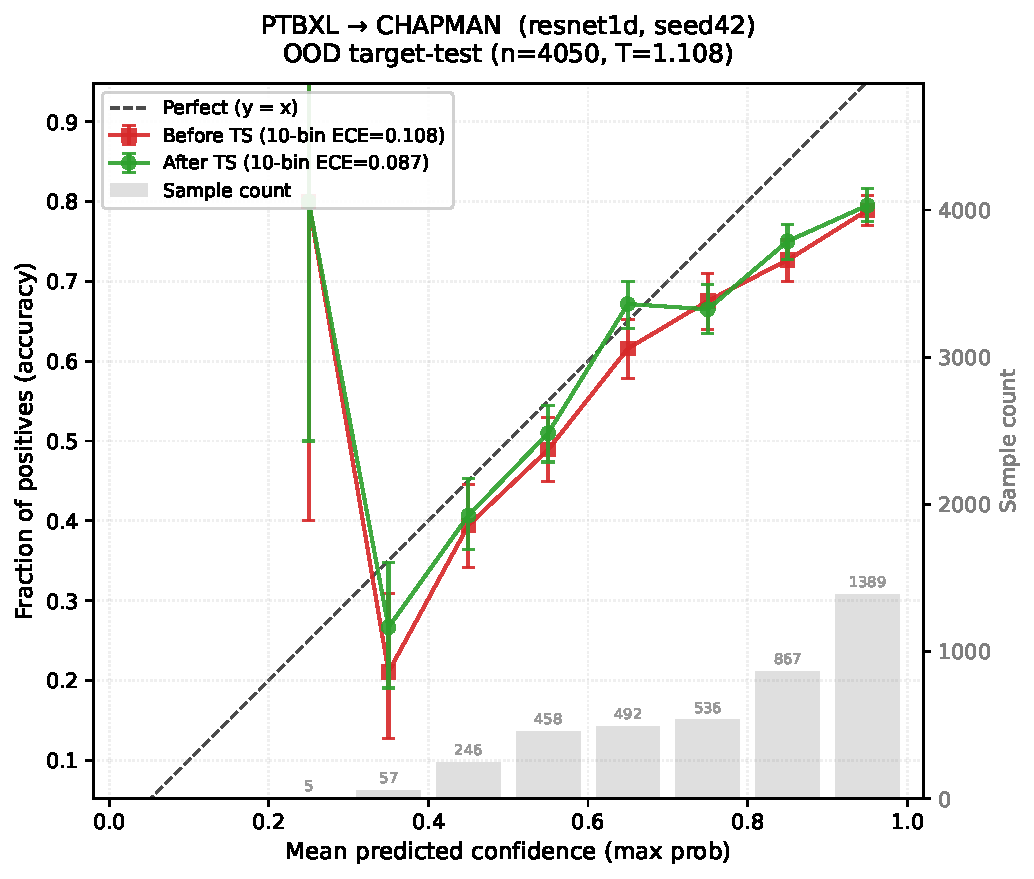
\includegraphics[width=0.32\textwidth]{figures/fig_reliability_supp_ptbxl_chapman_resnet1d_seed42.pdf}
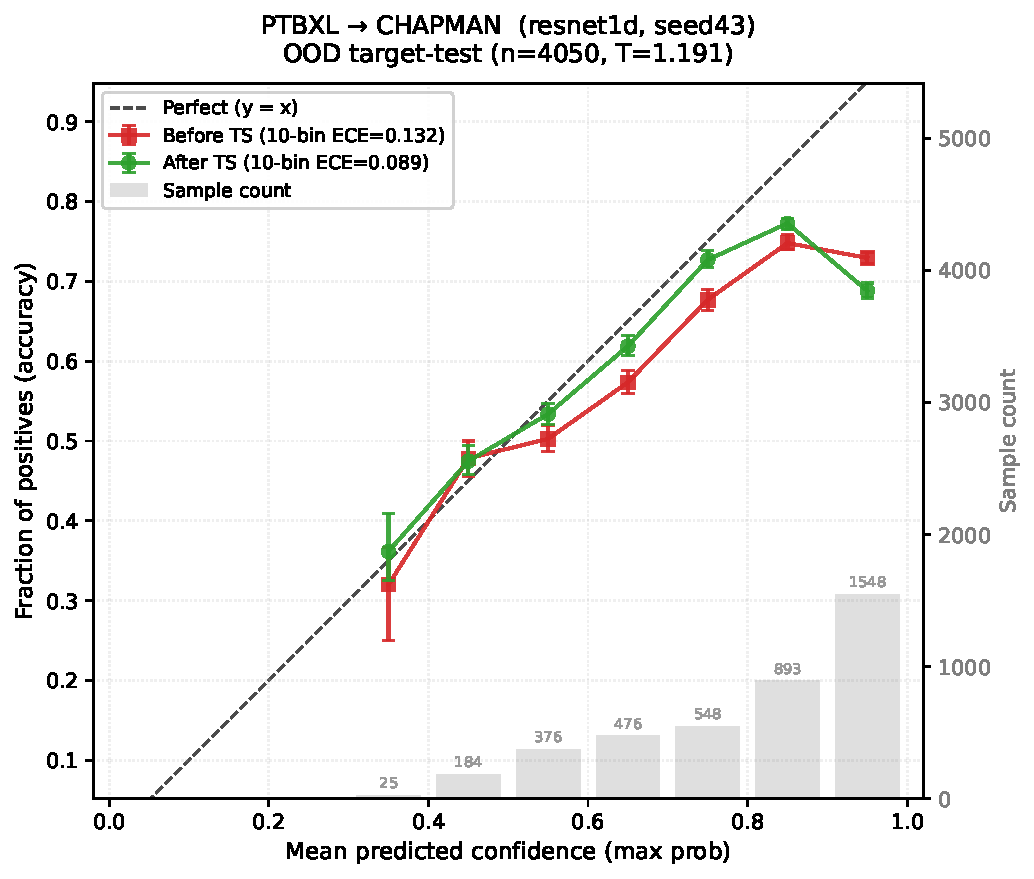
\includegraphics[width=0.32\textwidth]{figures/fig_reliability_supp_ptbxl_chapman_resnet1d_seed43.pdf}
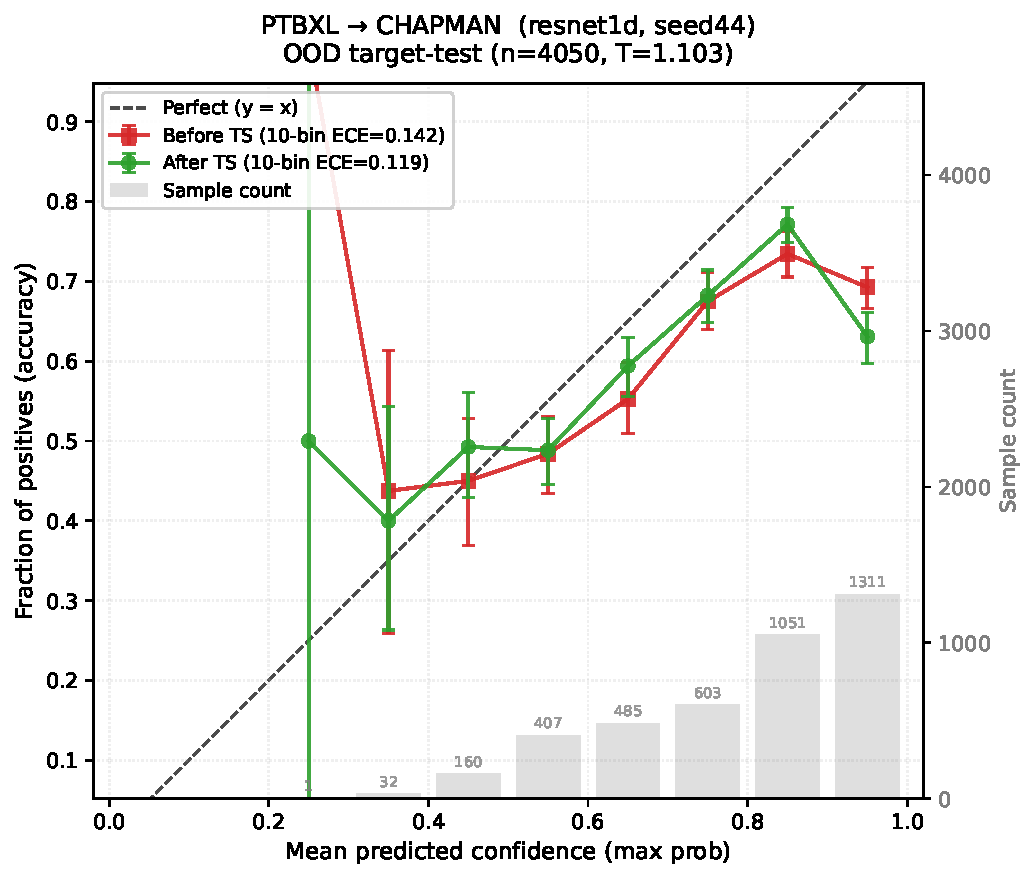
\includegraphics[width=0.32\textwidth]{figures/fig_reliability_supp_ptbxl_chapman_resnet1d_seed44.pdf}
\caption{PTB-XL$\to$Chapman 可靠性图：ResNet1D 种子 42--44。}
\end{figure}

\begin{figure}[h]
\centering
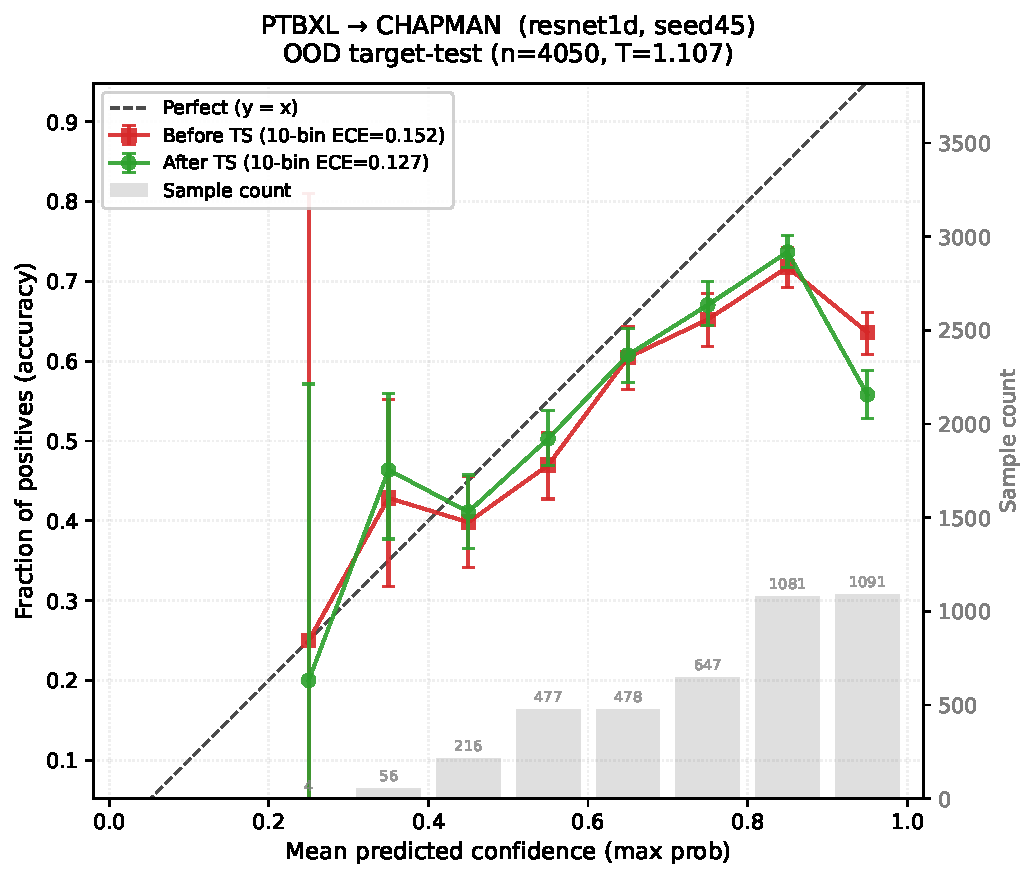
\includegraphics[width=0.45\textwidth]{figures/fig_reliability_supp_ptbxl_chapman_resnet1d_seed45.pdf}
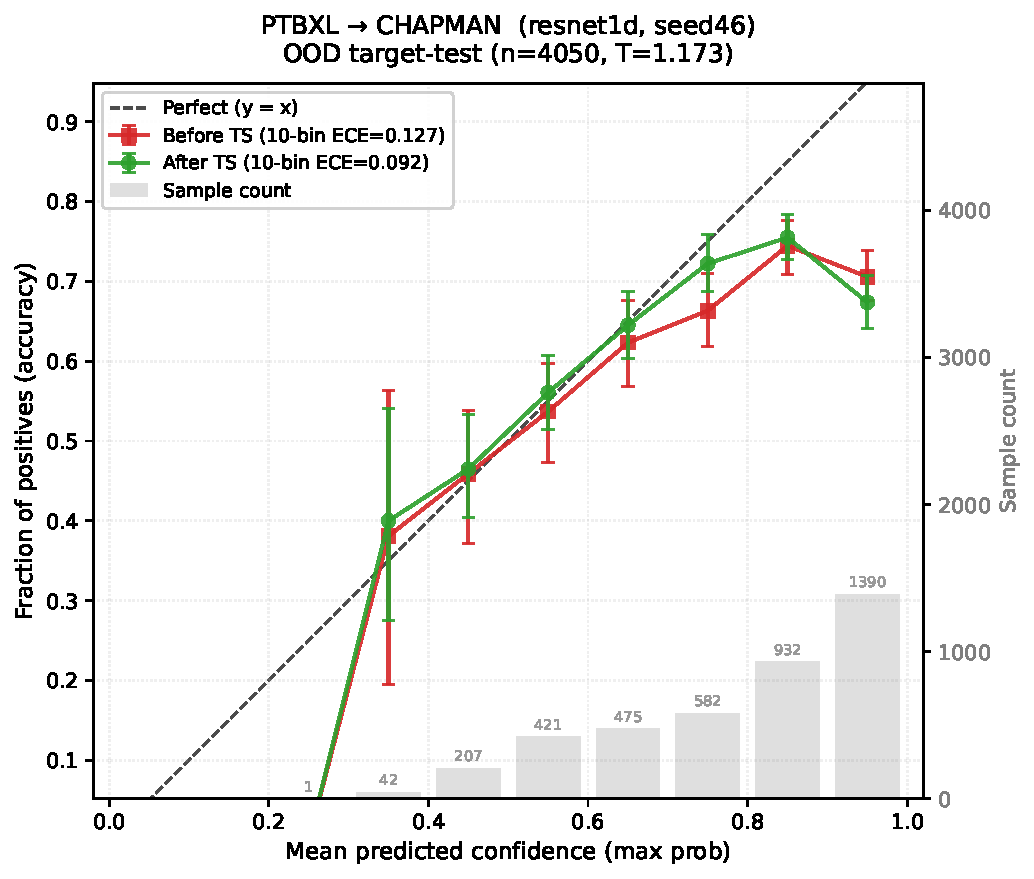
\includegraphics[width=0.45\textwidth]{figures/fig_reliability_supp_ptbxl_chapman_resnet1d_seed46.pdf}
\caption{PTB-XL$\to$Chapman 可靠性图：ResNet1D 种子 45--46。}
\end{figure}

\begin{figure}[h]
\centering
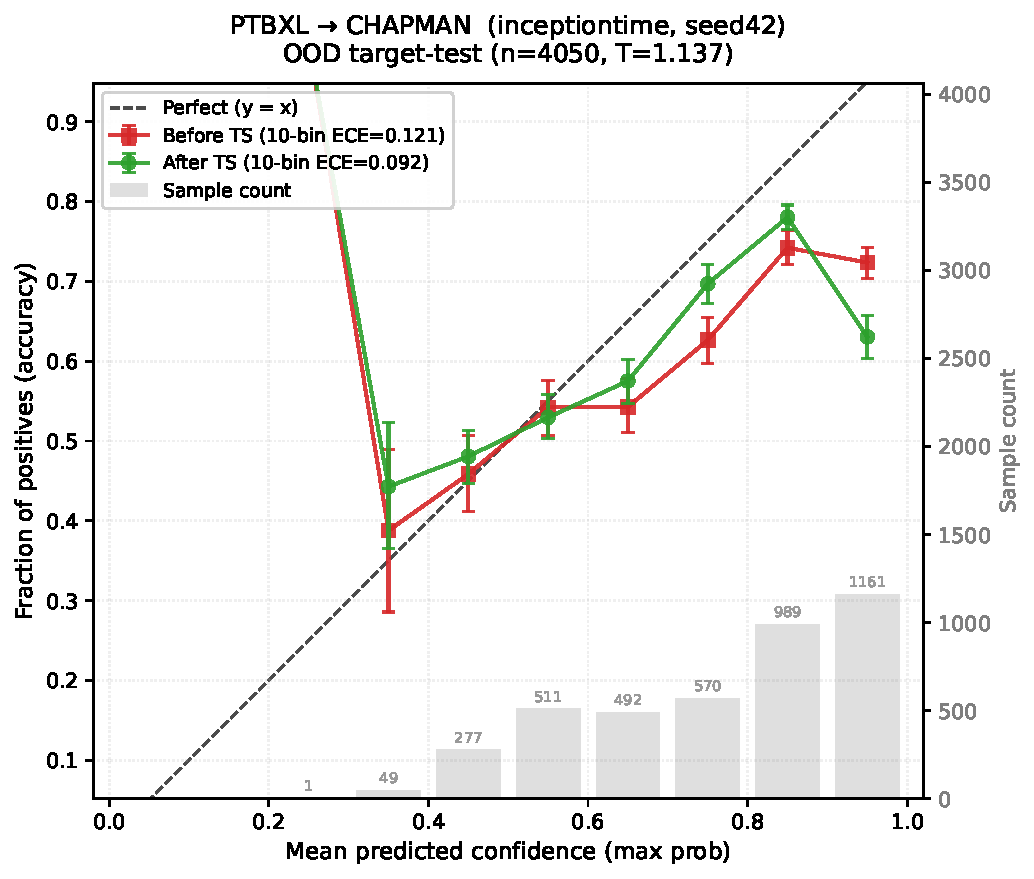
\includegraphics[width=0.32\textwidth]{figures/fig_reliability_supp_ptbxl_chapman_inceptiontime_seed42.pdf}
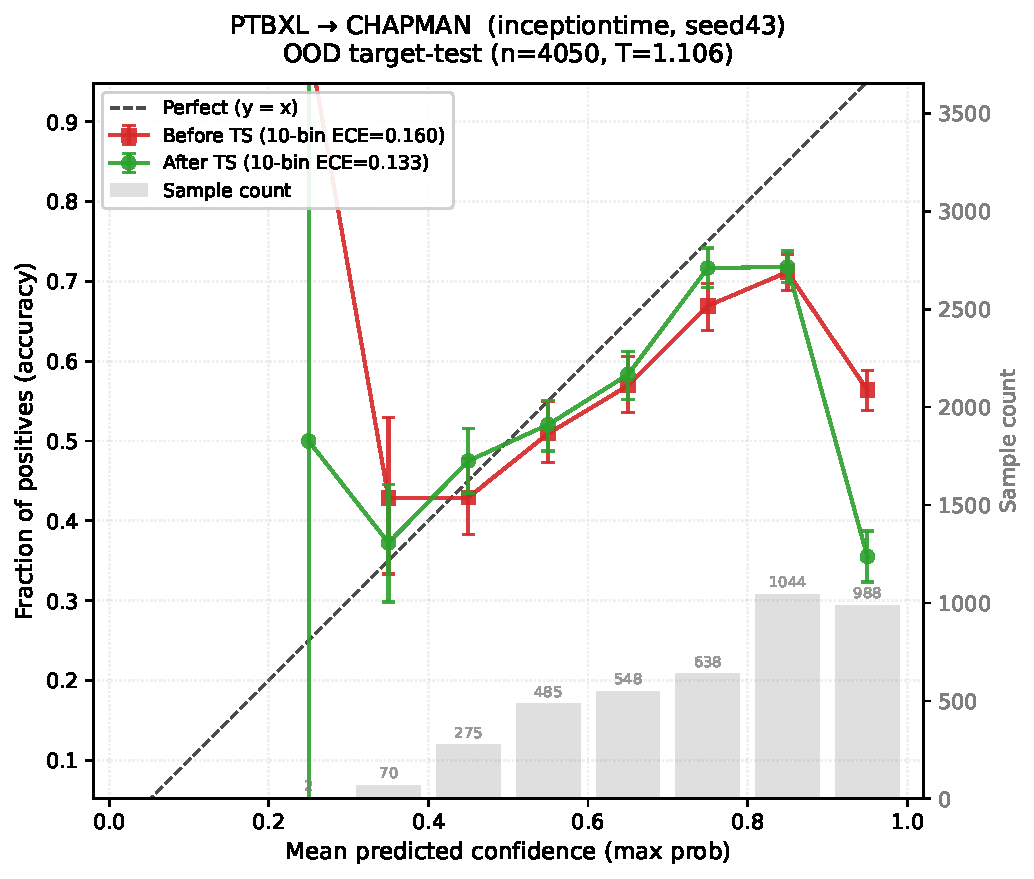
\includegraphics[width=0.32\textwidth]{figures/fig_reliability_supp_ptbxl_chapman_inceptiontime_seed43.pdf}
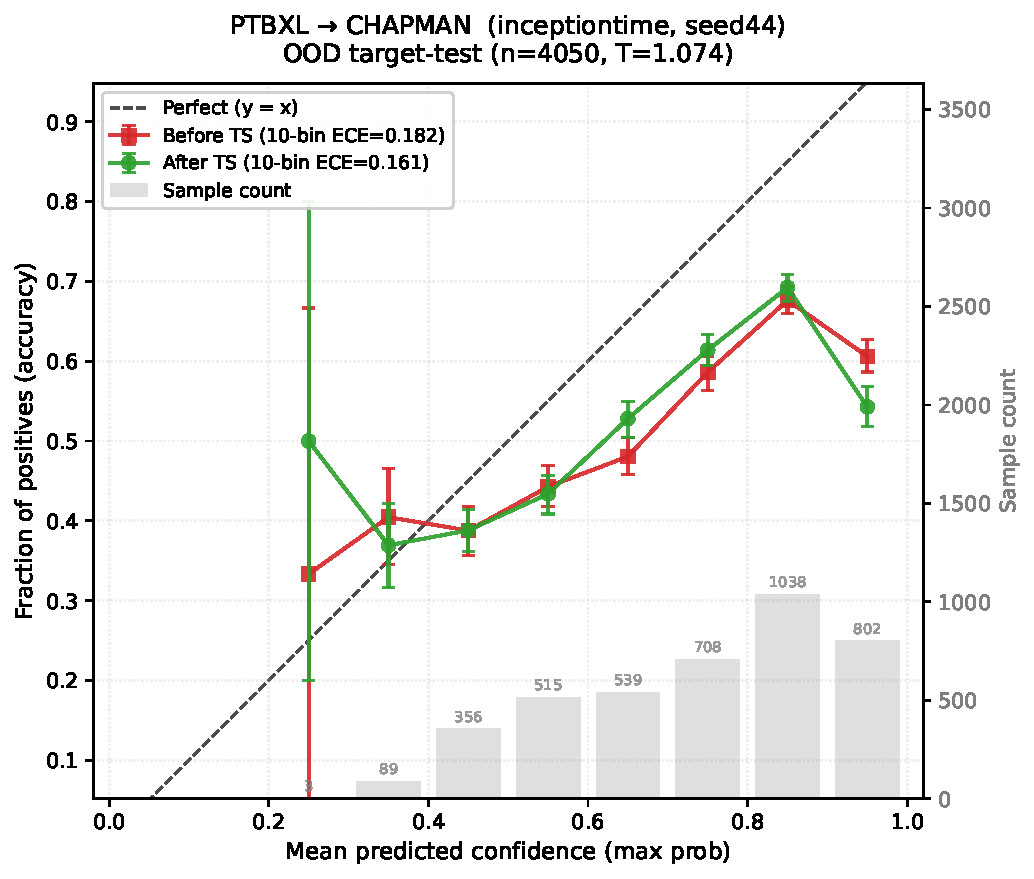
\includegraphics[width=0.32\textwidth]{figures/fig_reliability_supp_ptbxl_chapman_inceptiontime_seed44.pdf}
\caption{PTB-XL$\to$Chapman 可靠性图：InceptionTime 种子 42--44。}
\end{figure}

\begin{figure}[h]
\centering
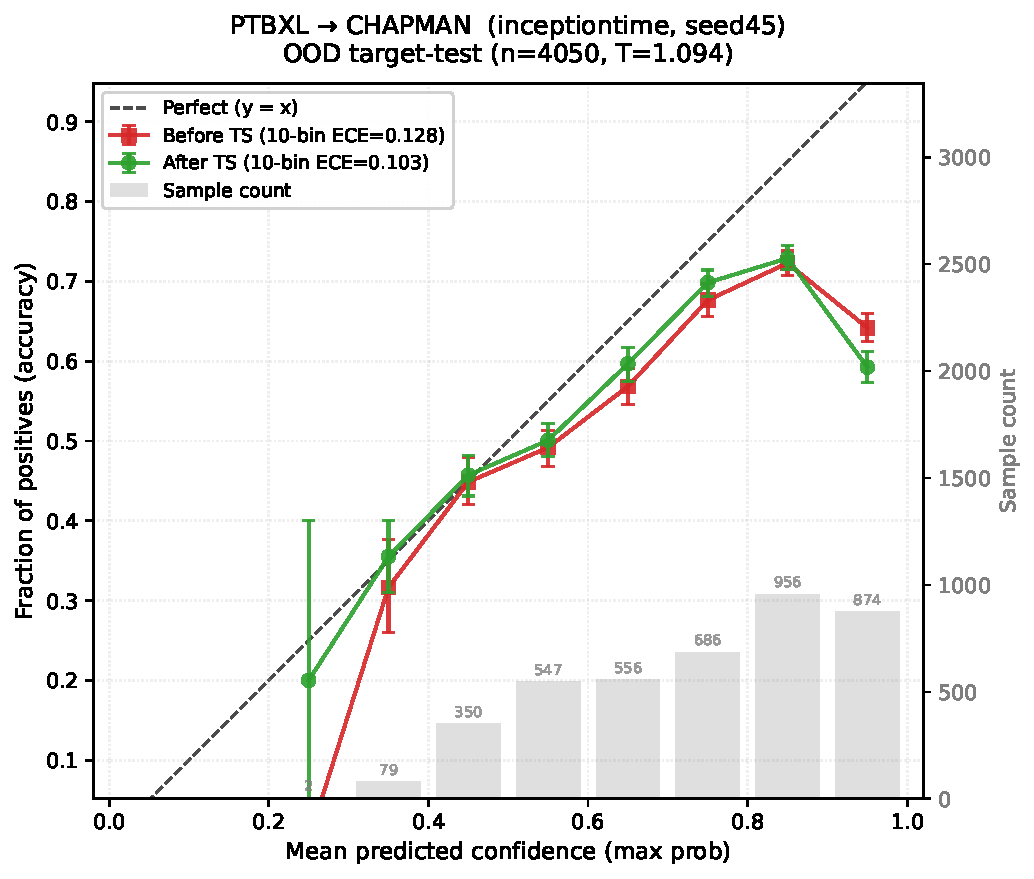
\includegraphics[width=0.45\textwidth]{figures/fig_reliability_supp_ptbxl_chapman_inceptiontime_seed45.pdf}
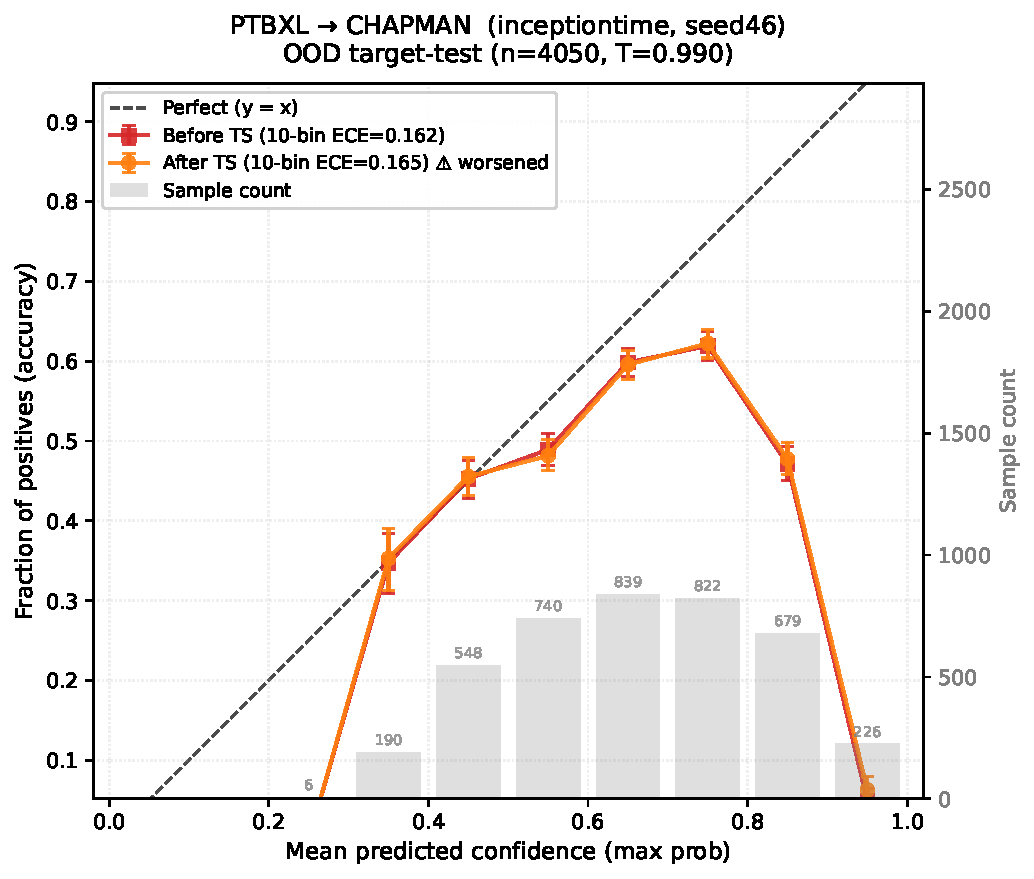
\includegraphics[width=0.45\textwidth]{figures/fig_reliability_supp_ptbxl_chapman_inceptiontime_seed46.pdf}
\caption{PTB-XL$\to$Chapman 可靠性图：InceptionTime 种子 45--46。}
\end{figure}

\subsubsection*{S1.6.\ PTB-XL$\rightarrow$CPSC}

\begin{figure}[h]
\centering
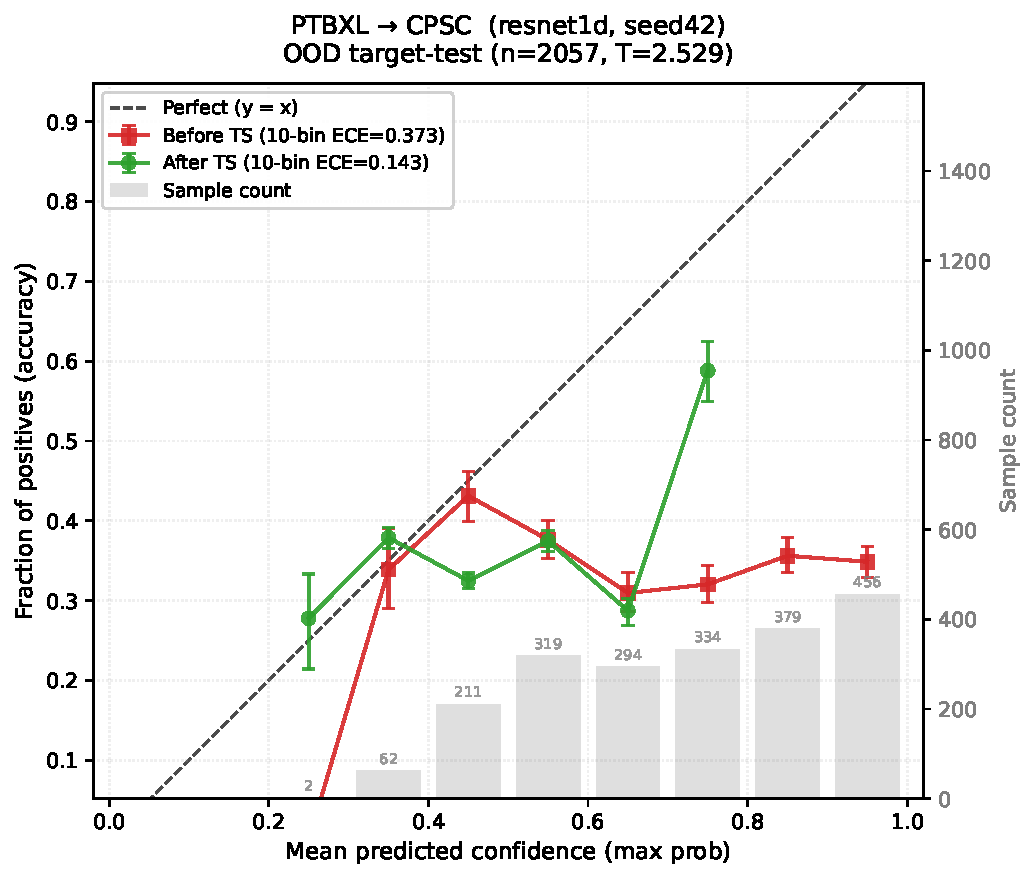
\includegraphics[width=0.32\textwidth]{figures/fig_reliability_supp_ptbxl_cpsc_resnet1d_seed42.pdf}
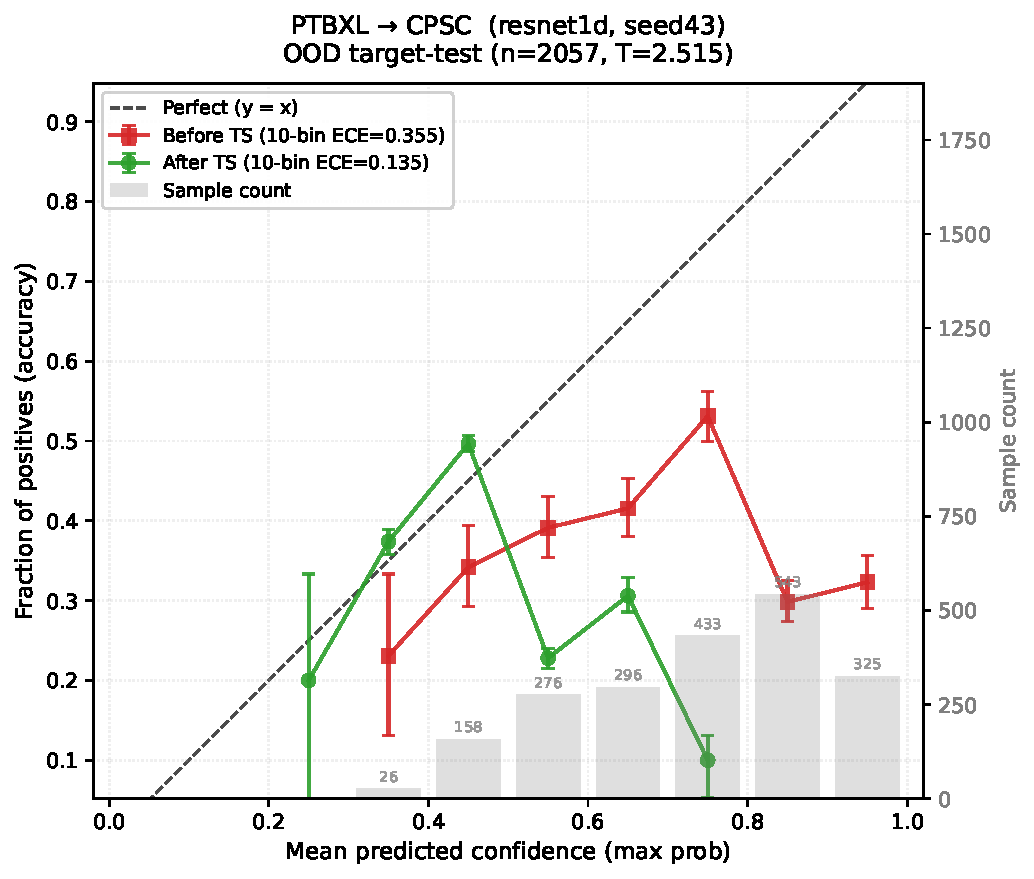
\includegraphics[width=0.32\textwidth]{figures/fig_reliability_supp_ptbxl_cpsc_resnet1d_seed43.pdf}
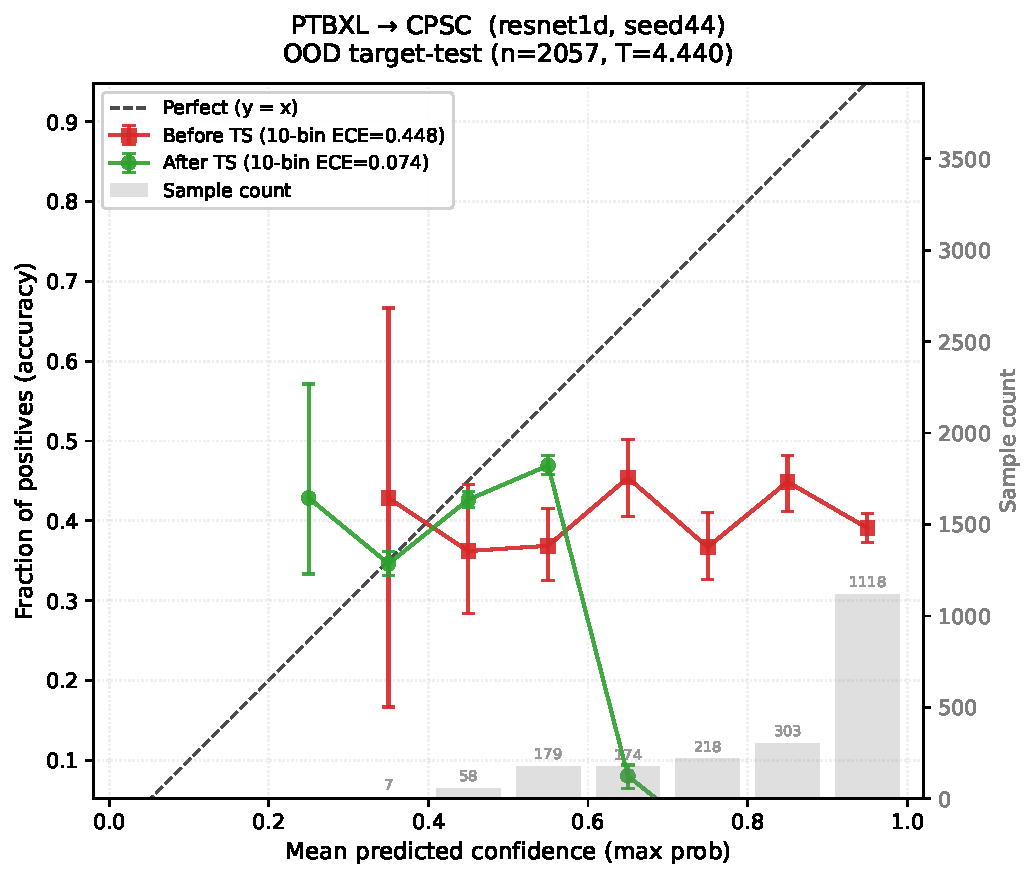
\includegraphics[width=0.32\textwidth]{figures/fig_reliability_supp_ptbxl_cpsc_resnet1d_seed44.pdf}
\caption{PTB-XL$\to$CPSC 可靠性图：ResNet1D 种子 42--44。}
\end{figure}

\begin{figure}[h]
\centering
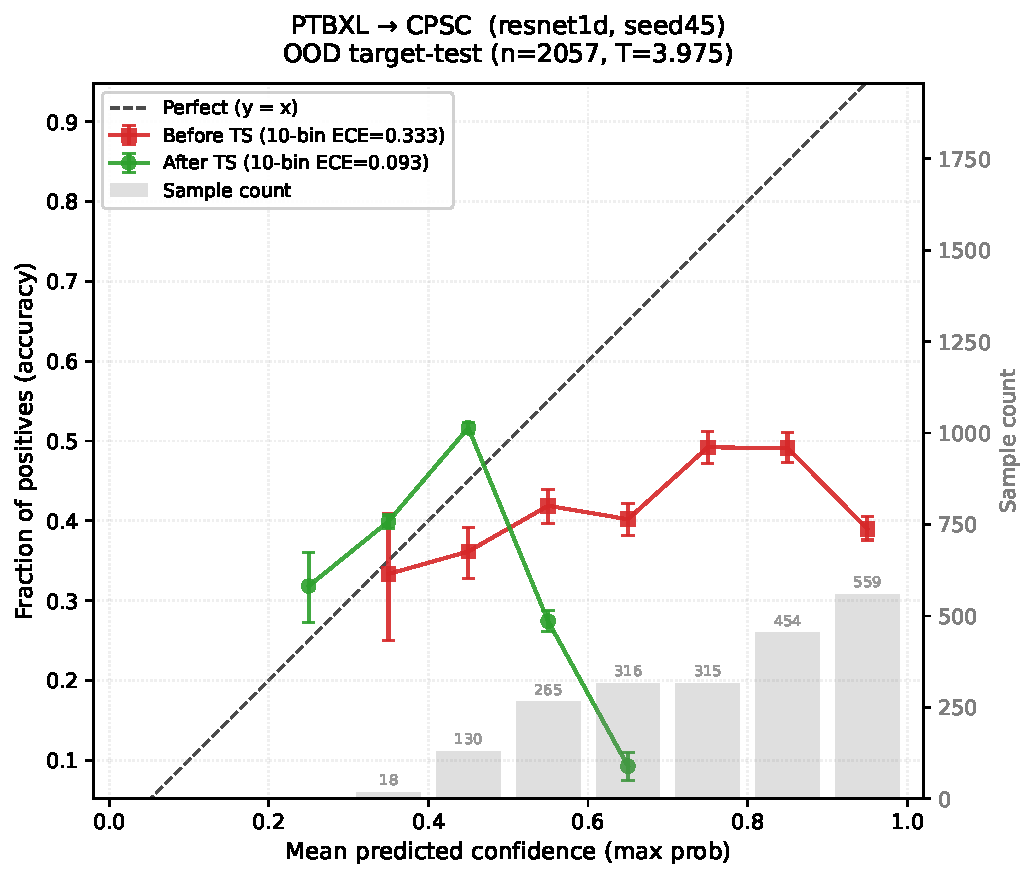
\includegraphics[width=0.45\textwidth]{figures/fig_reliability_supp_ptbxl_cpsc_resnet1d_seed45.pdf}
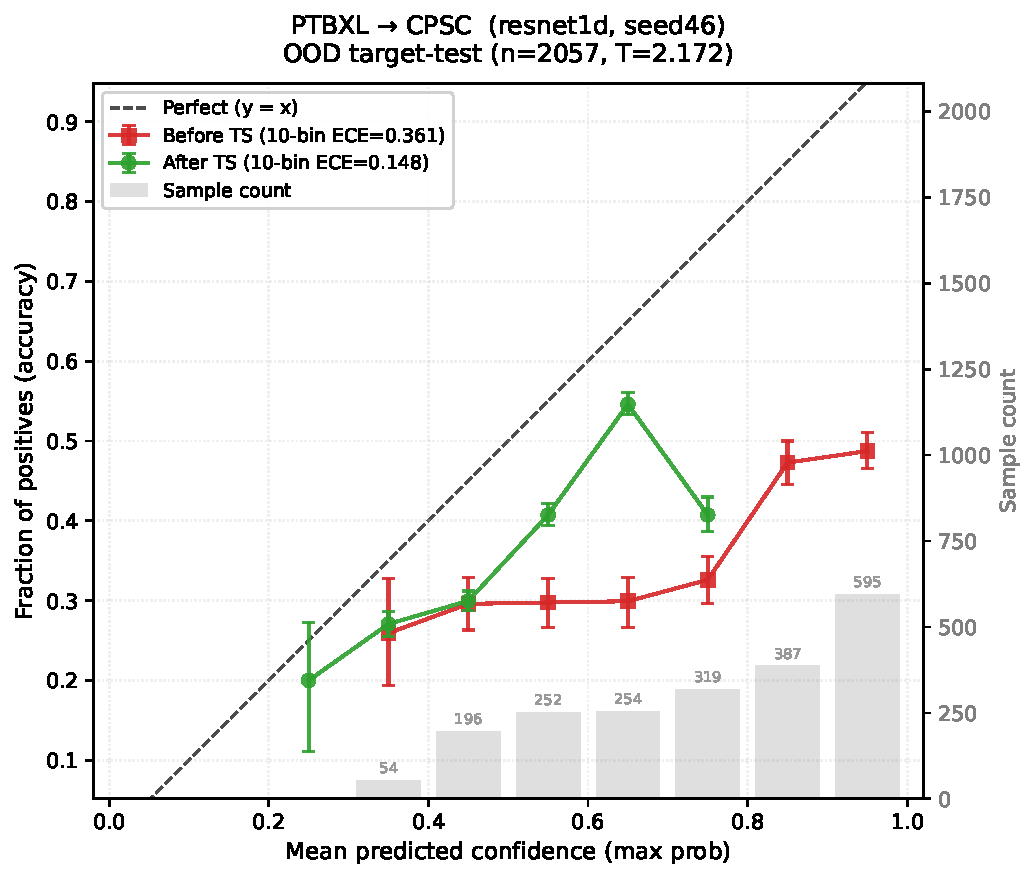
\includegraphics[width=0.45\textwidth]{figures/fig_reliability_supp_ptbxl_cpsc_resnet1d_seed46.pdf}
\caption{PTB-XL$\to$CPSC 可靠性图：ResNet1D 种子 45--46。}
\end{figure}

\begin{figure}[h]
\centering
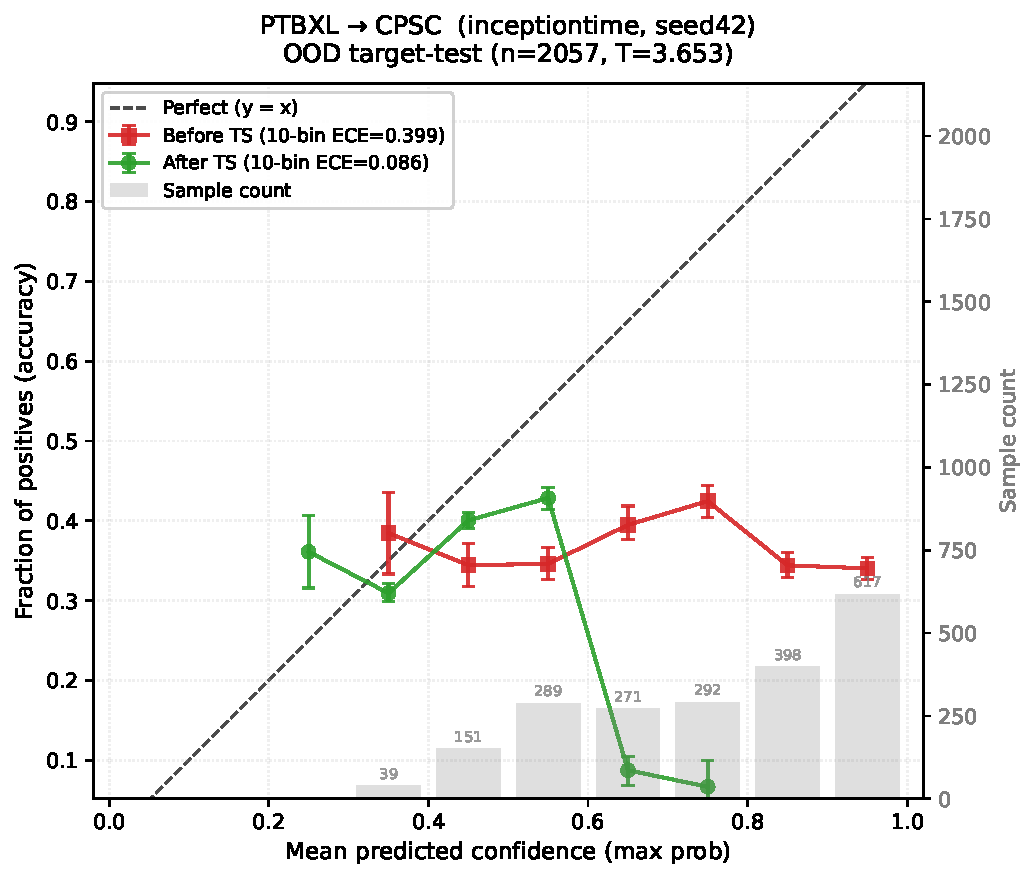
\includegraphics[width=0.32\textwidth]{figures/fig_reliability_supp_ptbxl_cpsc_inceptiontime_seed42.pdf}
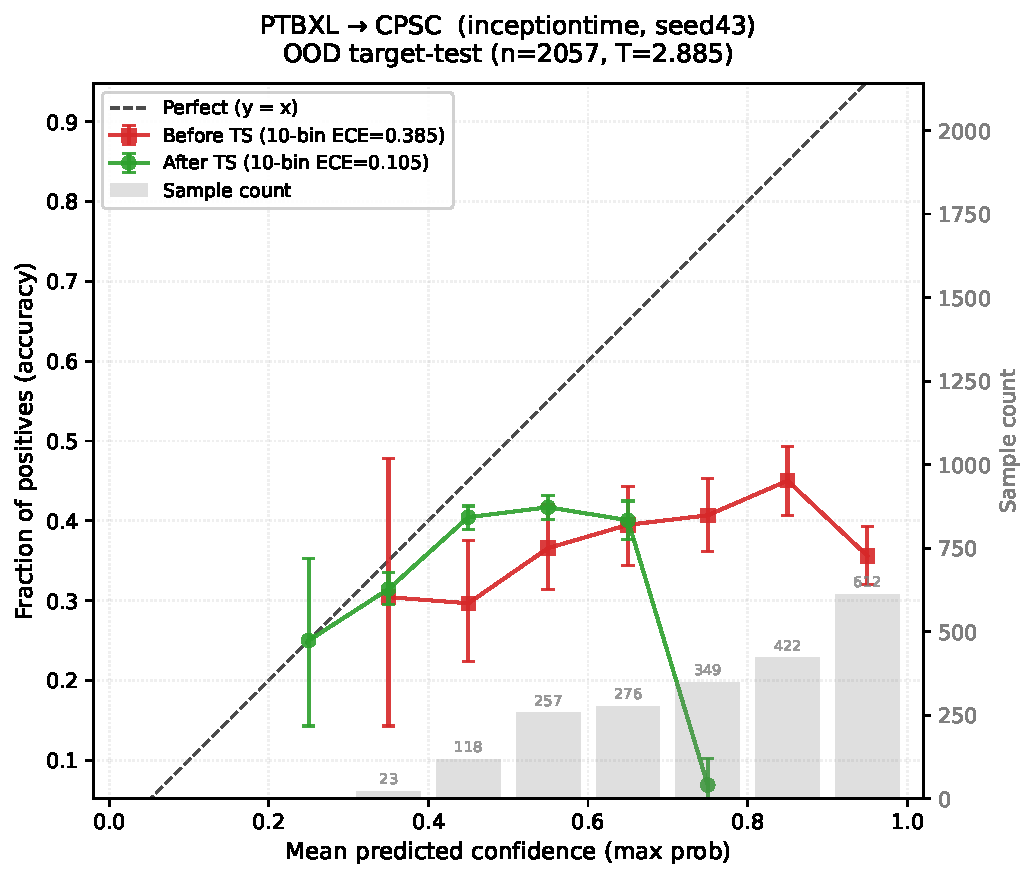
\includegraphics[width=0.32\textwidth]{figures/fig_reliability_supp_ptbxl_cpsc_inceptiontime_seed43.pdf}
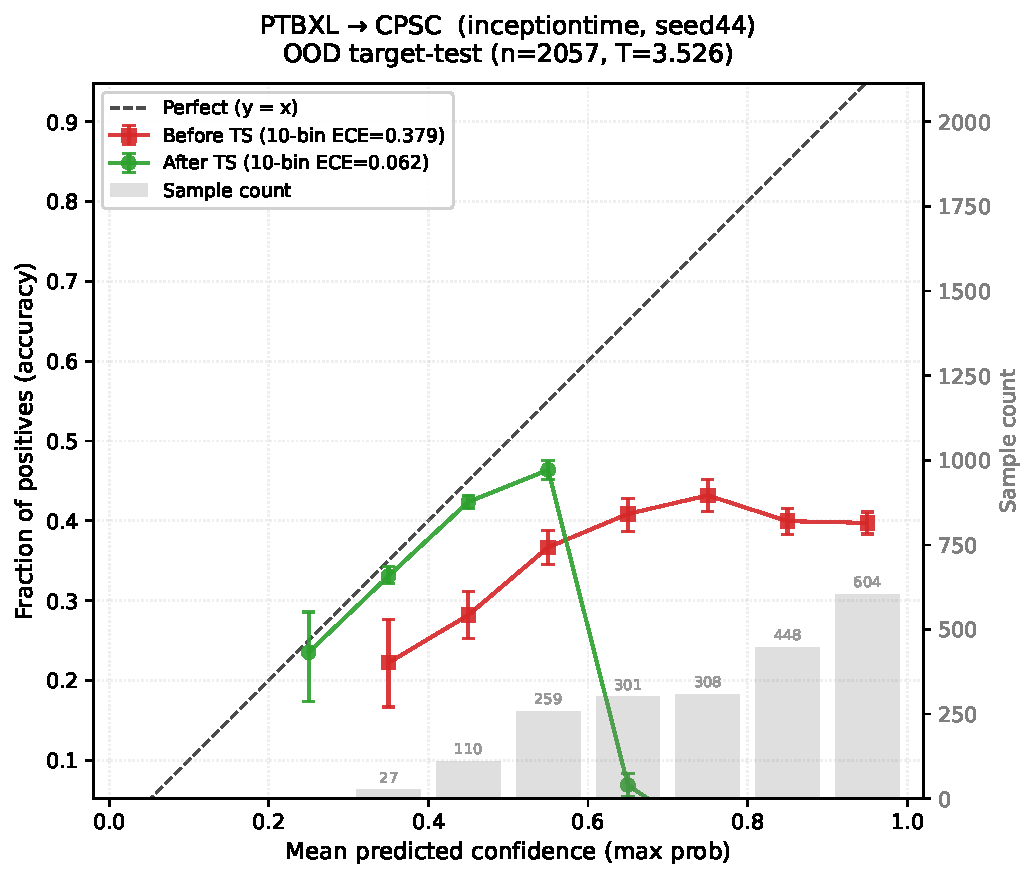
\includegraphics[width=0.32\textwidth]{figures/fig_reliability_supp_ptbxl_cpsc_inceptiontime_seed44.pdf}
\caption{PTB-XL$\to$CPSC 可靠性图：InceptionTime 种子 42--44。}
\end{figure}

\begin{figure}[h]
\centering
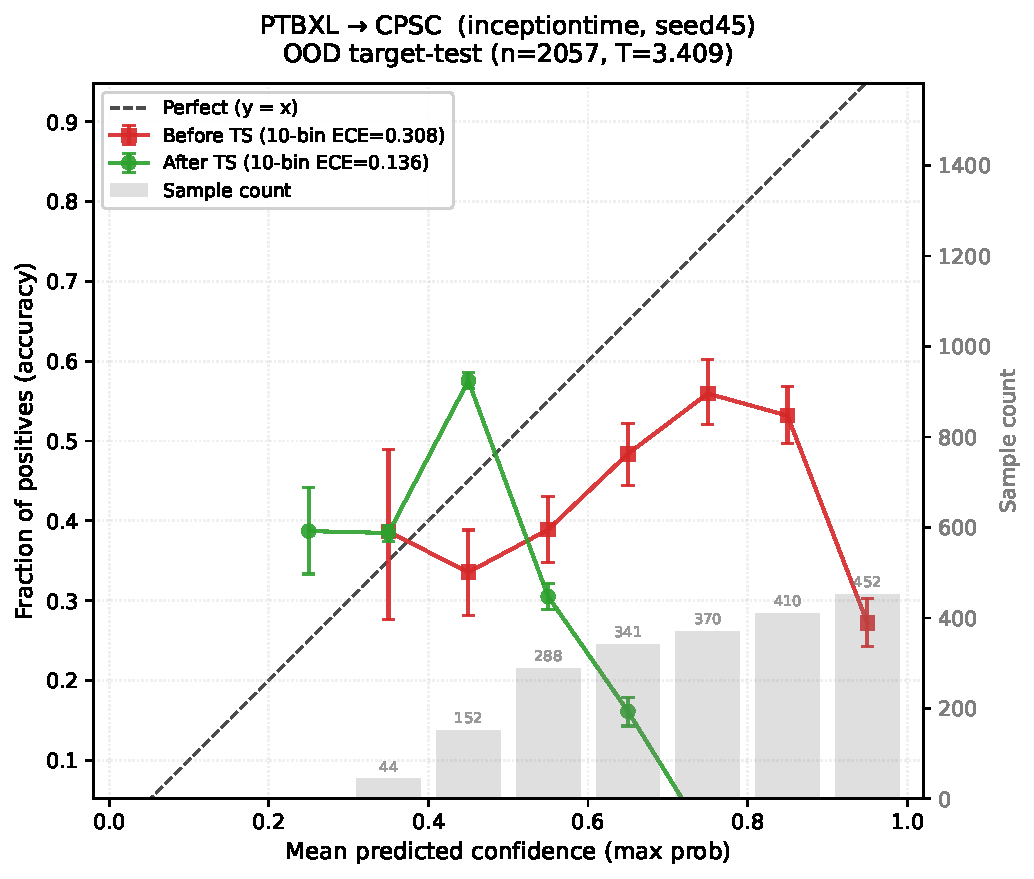
\includegraphics[width=0.45\textwidth]{figures/fig_reliability_supp_ptbxl_cpsc_inceptiontime_seed45.pdf}
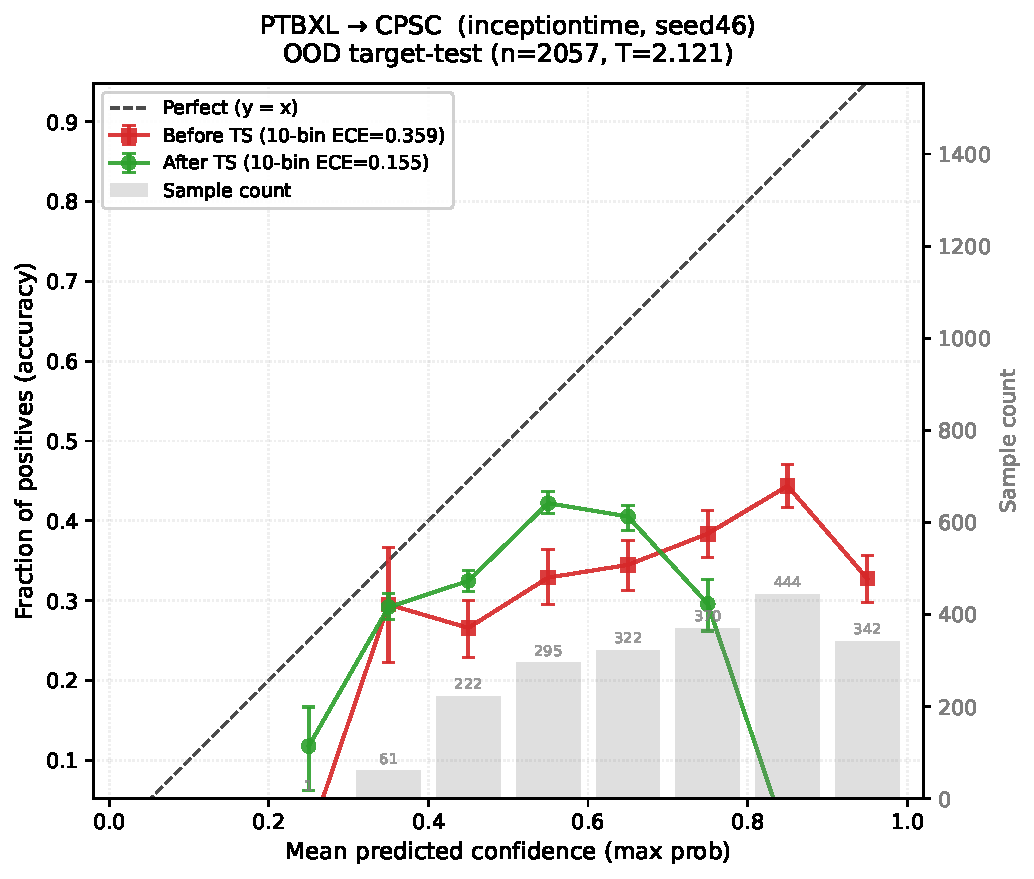
\includegraphics[width=0.45\textwidth]{figures/fig_reliability_supp_ptbxl_cpsc_inceptiontime_seed46.pdf}
\caption{PTB-XL$\to$CPSC 可靠性图：InceptionTime 种子 45--46。}
\end{figure}

\subsection*{S2.\ 其他补充材料}
\label{sec:supp-additional}
\begin{itemize}
    \item \textbf{逐实验结果文件}：全部 60 个种子实验的完整 JSON 结果
    （\texttt{checkpoints/transfer/**/}\allowbreak\texttt{transfer\_result.json}）
    和 CSV 汇总（\texttt{results/*.csv}）。
    \item \textbf{预注册协议}：修订版 A1 全文
    （\texttt{docs/PROTOCOL\_AMENDMENT\_A1\_}\allowbreak\texttt{PREREG\_RELOCATION.md}）
    和哈希清单（\texttt{docs/osf\_archive\_manifest.json}）。
    \item \textbf{NCV 实验数据}：包含净临床价值实验（Section~\ref{sec:ncv_methods}）
    所用 \texttt{ncv\_id} 和 \texttt{ncv\_ood} 列的 E3 CSV 文件。
    \item \textbf{Shapley 分解单元}：用于 $n=20{,}000$ 处 Shapley 归因分析的
    27 单元验证表。
    \item \textbf{BCa 置信区间重算清单}：整个 $6 \times 2 \times 5 \times 8$
    网格的完整 BCa 自助法（$B=10{,}000$）置信区间结果，存储于每个
    \texttt{transfer\_result.json} 的 \texttt{methods.ts.meta} 字段中。
\end{itemize}
